
\subsection{Investigative Approach: User-centered Participatory Design}
Our previous work in accessible mobility and transit as well as in building information technology to communicate and close the informational gaps experienced by travelers with special needs led us to develop a holistic approach to measuring “accessibility of the full travel chain,” involving coordination between transportation departments and peers in human service departments, and also involving participatory design principles (in which an active group of participants from the population of interest, in our case individuals who are Deaf-blind and their supporters, actively participate in the design process). We have employed a specific user-empowerment design methodology, and a nuanced model of ‘accessibility’ which takes into account the fact that ‘disability’ is an umbrella term for a truly heterogeneous population and that effective mobility and transit solutions for such a variable population requires inherent flexibility and customization. This approach guides the development iterations, validation, analysis steps, and coordination that our team will implement to ensure successful, comprehensive, value-sensitive design iterations.

The UW team is partnering with the City of Seattle Title II ADA Compliance Program to pursue development and pilot testing of a prototype Tactile Map Tile application in Seattle. To date, TCAT has an excellent working relationship with the City of Seattle. Additionally, Seattle's Lighthouse for the Blind makes an ideal local partner because of its ongoing commitment to accessibility and continual innovation for the city's blind and Deaf-blind population. The AccessMap and OpenSidewalks Projects are both examples of TCAT's commitment to accessibility through partnerships. 

To ensure the success of the Tactile Map Tile development project, we developed two core teams of stakeholders: the Technical Team and the Community of Practice Group (stakeholder group). While some staff resources are shared between the two groups, in the three year development period, we intend to pursue continuous iteration between achieving planned technical goals (described in the development activities in Sections \ref{sec:fabrication}-\ref{sec:alerts}) and learning from real-use evaluation (described in the data collection and community activities in Section \ref{sec:stakeholder-input}).
Therefore, the technical development tasks should be sometimes concurrently occurring with validation testing and translation to practice. This will allow us to outline a process that enables  faster prototyping iterations, mutual learning, including collective reflection-in-action, through trial use of the tactile maps for various trip purposes. In our experience, this type of development allows for emergent and opportunity-based changes to the technical design resulting from trial use of new maps by the Community of Practice. 


\label{sec:approach}


The Tactile Map Tile concept builds on existing technology and research to combine \textit{additive manufacturing} (3D printing) and \textit{relevant pedestrian pathway details} to resolve a significant unmet communication need  for the Deaf-blind cohort. A single‐endpoint integration of these tools has yet to be piloted, tested or proven.  Our main challenge in translating this integration to active use in the field is to develop tactile informational encodings that simultaneously allow independent travel and are simple, clear  and pleasant to use via touch. 

%(i) The extent to which the proposed project methodology is meritorious, including consideration of the extent to which: (A) The proposed project shows awareness of the state-of-the-art for current, related products. (B) The proposed project employs appropriate concepts, components, or systems to develop the new or improved product. (C) The proposed project employs appropriate samples in tests, trials, and other development activities. (D) The proposed project conducts development activities in appropriate environment(s). (E) Input from individuals with disabilities and other key stakeholders is obtained to establish and guide proposed development activities. (F) The applicant identifies and justifies the stage(s) of development for the proposed project; and activities associated with each stage. 

Above, we have delineated six development activity objectives necessary to satisfy our design criteria. We now describe each activity, including state-of-the-art, related work and the development and validation activities needed to incorporate it into our solution. To ensure usability of our design, we will pursue participatory design practices throughout all development activities. 
%To highlight the participatory design work, each of the development activities will incorporate a section about design activities, detailing the design explorations and tests we will undertake in natural environments. \ac{if there's time add this}
Finally, we map each activity to one of our three key deliverables: accessible web interfaces, algorithms for creating custom tactile maps, and a printing and update notification system.

Our development activities focus on iterative refinement of the
three main threads of the work, namely the development of high quality
optimal tangible maps, the development of a web interface that
empowers Deaf-blind individuals to requisition their own maps on the
fly and a subscription service to updates about the area of interest to travelers. Stakeholder input activities (described in Section \ref{sec:stakeholder-input}) will be weaved-in throughout the development of the project to offer interim and development product validation. Our Workplan (Section \ref{sec:workplan}) will describe the development flow in greater detail.

\subsection{Form Factor: Tangible Map Design Using Additive Manufacturing (3D printing)}
This section describes development activities associated with integrating the relevant map information in the right form factor. Specifically, the development activity of producing an automated pipeline to produce 3D print model of a tcatile map is the first part of delivering tangible map design (Product 1). A 3D printed solution is suitable for our user population, ensuring it relays mobility information in a non-visual, non-auditory manner, but is also affordable, cost-effective, scalable and reproducible.  The importance of bringing down the cost and increasing accessibility of tactile maps is discussed.

Development goal: Extending our aggregated accessibility map codebase to support a production-level pipeline that produces 3D printed map models thereby extending reach and scalability (while reducing costs) of tactile maps.  

\label{sec:fabrication}
%(i) The extent to which the proposed project methodology is meritorious, including consideration of the extent to which: (A) The proposed project shows awareness of the state-of-the-art for current, related products. (B) The proposed project employs appropriate concepts, components, or systems to develop the new or improved product. (C) The proposed project employs appropriate samples in tests, trials, and other development activities. (D) The proposed project conducts development activities in appropriate environment(s). (E) Input from individuals with disabilities and other key stakeholders is obtained to establish and guide proposed development activities. (F) The applicant identifies and justifies the stage(s) of development for the proposed project; and activities associated with each stage. 

\subsubsection{Background and State-of-the-Art}

\textbf{Non visual Navigational Aids}

Tool development for low vision and blind populations has ranged from audible navigational aids, to smart canes and wearable technologies that can communicate with instrumented environments providing enhanced information to pedestrians as they travel through a space. 

In contrast, maps have potentially richer content. Indeed, maps are an important tool for  navigation because they help people to understand the spatial layout of the targeted environment. However, most maps are inherently visual. One solution that has a long history in the Blind and Blind-deaf community is tactile maps. Common approaches include embossing, printing ind Braille, and "swell" (microcapsule) paper. These approaches can be used to create a two-layer tactile visualization from an image (\textit{e.g.}, \cite{miele2006talking}). However such machines can be very costly \cite{rice2005design}, are not readily available, and lack the expressive range of a solution that can vary more in height. While vacuum-forming has more height, it depends on a pre-existing form, which limits its customizability. Finally, the design of a tactile map requires expertise to be easily understandable \cite{tatham1991design}.


\textbf{Tactile Maps}

The utility of tactile maps in wayfinding and orientation for people with visual impairments is well established. Tactile maps provide users with information that facilitates enhanced orientation and navigation (Erin 2009; Espinosa et al. 1998), while also giving form to the pedestrian environments that impact the way everyone moves through space. 
Tactile maps have been demonstrated to contribute to people’s ability to learn new routes, and are an important source of geographical information, particularly when people are learning new environments (Blades, Ungar, and Spencer 1999). 

As with graphic maps, there a variety of ways in which tactile maps can be used.  When compared to a group that received a verbal description, blind and low vision pedestrians were shown to gain significantly more spatial knowledge by experiencing a new urban environment with a tactile map (Espinosa et al. 1998).   Tactile maps provide an opportunity for users to orient in urban and rural environments (Rowell and Ungar 2003c), as well as in more confined spaces such as buildings, conference centers or campuses (Erin 2009).  These physical representations of the environment can be used while actively navigating or orienting, but also facilitate learning a route prior to embarking on a journey (Espinosa et al. 1998).  Due to a lack of experience with tactile maps not all people that are blind or have low vision feel comfortable using this type of navigational aid (Erin 2009).  However, tactile graphics are generally accepted as useful for providing contextual information that is not directly related to mobility, such as city’s location within a state (Erin 2009).

\textbf{Fabricated Tactile Maps}

As noted earlier, traditional production methods can be very costly \cite{rice2005design}, difficult to reproduce, non-scalable, and the technology for creating these artifacts are not readily available. 3D printing, also called consumer-grade manufacturing, is ideally suited for bringing  down costs when customization is needed. 3D printers are now available for a price point  as low as 200 dollars, and services that 3D print any valid file are also widely available. Thus,  3D printing is democratizing access to manufacturing of tangible, physical objects. 


Despite  indications that improving mass fabrication techniques for the production of tactile maps 
could be beneficial for people with both visual and hearing loss, this area remains relatively unexplored in contrast to the body of work on mobile navigation apps and other connected devices that serve as navigational aids. Recent work has begun to explore the use of 3D 
printing to reduce cost. 
For example, it is now possible to requisition a custom, laser-cut topographical map on ETSY \cite{etsy} or purchase custom 3D printed topographic models through companies such as Sightline \url{sightlinemaps.com} or PrintMyRoute \url{www.printmyroute.xyz}. 

The accessibility community has added its own spin to these technologies. For example TouchMapper \textit{touch-mapper.org} is a free service that will create a tactile map using embossing or 3D printing and help connect you to existing online printing services or print it yourself.  This service focuses on showing streets, and can be customized for size, inclusion of buildings and some other features. However it too does not include route finding or landmark identification. There are additional issues with the approach since the maps do not designate topography, do not represent pedestrian-centric information (such as what type of pedestrian signal is at a crossing), nor other important environmental representations that would allow a traveler who is blind or Deaf-blind make informed decisions about choosing a route. 
Specifically, the services do not include features intended to support Deaf-blind users, and do not support travel activities such as route finding and landmark identification as a result. Other than our preliminary participant study, we are not aware that these systems have been tested with Deaf-blind individuals.


To summarize, tactile maps are not new to the cartographic record. Their value in facilitating orientation and navigation for the low vision and blind communities has been well established. However, their scope and availability has been greatly limited in the past by high production costs and limited interest from fields traditionally invested in map making and design.  3D printing has significantly reduced the costs of producing such maps, but to our knowledge no existing product has enhanced 3D printed maps with optimization and customization, making our product an important addition to this space. 


\subsubsection{Previous Development}

Our previous development focused on finding usable abstractions in the map to increase map content and user understanding of the pedestrian environment \ac{cite ASLA 2017}.
It is important to note that in our pilot work (Section \ref{sec:pilot}) users found the pedestrian environment more legible when the 3D printed maps did not directly model 1:1 the environments they represented. The greatest success with users (as measured by their later explanation of their mental model of the area) was perceived with maps that abstracted some features and omitted others in order to emphasize the information deemed important in the pedestrian environment. More space for the pedestrian information of interest was created through the reduction of building footprints by 70\% , and indenting the  them from the base rather than extruding. This still allowed users to understand the global form of the landscape, identify the buildings, and still incorporate rich information about sidewalks and intersections.


\subsubsection{Proposed Development}

We have a pipeline to create fabricated tactile maps that currently requires manual interventions. The work task for this development activity is to completely automate this workflow, as shown on the right side of Figure \ref{fig:TactileMapTileDev}.

\ac{explain the development activity of making the pipeline automated in words}

\begin{figure}
    \centering
    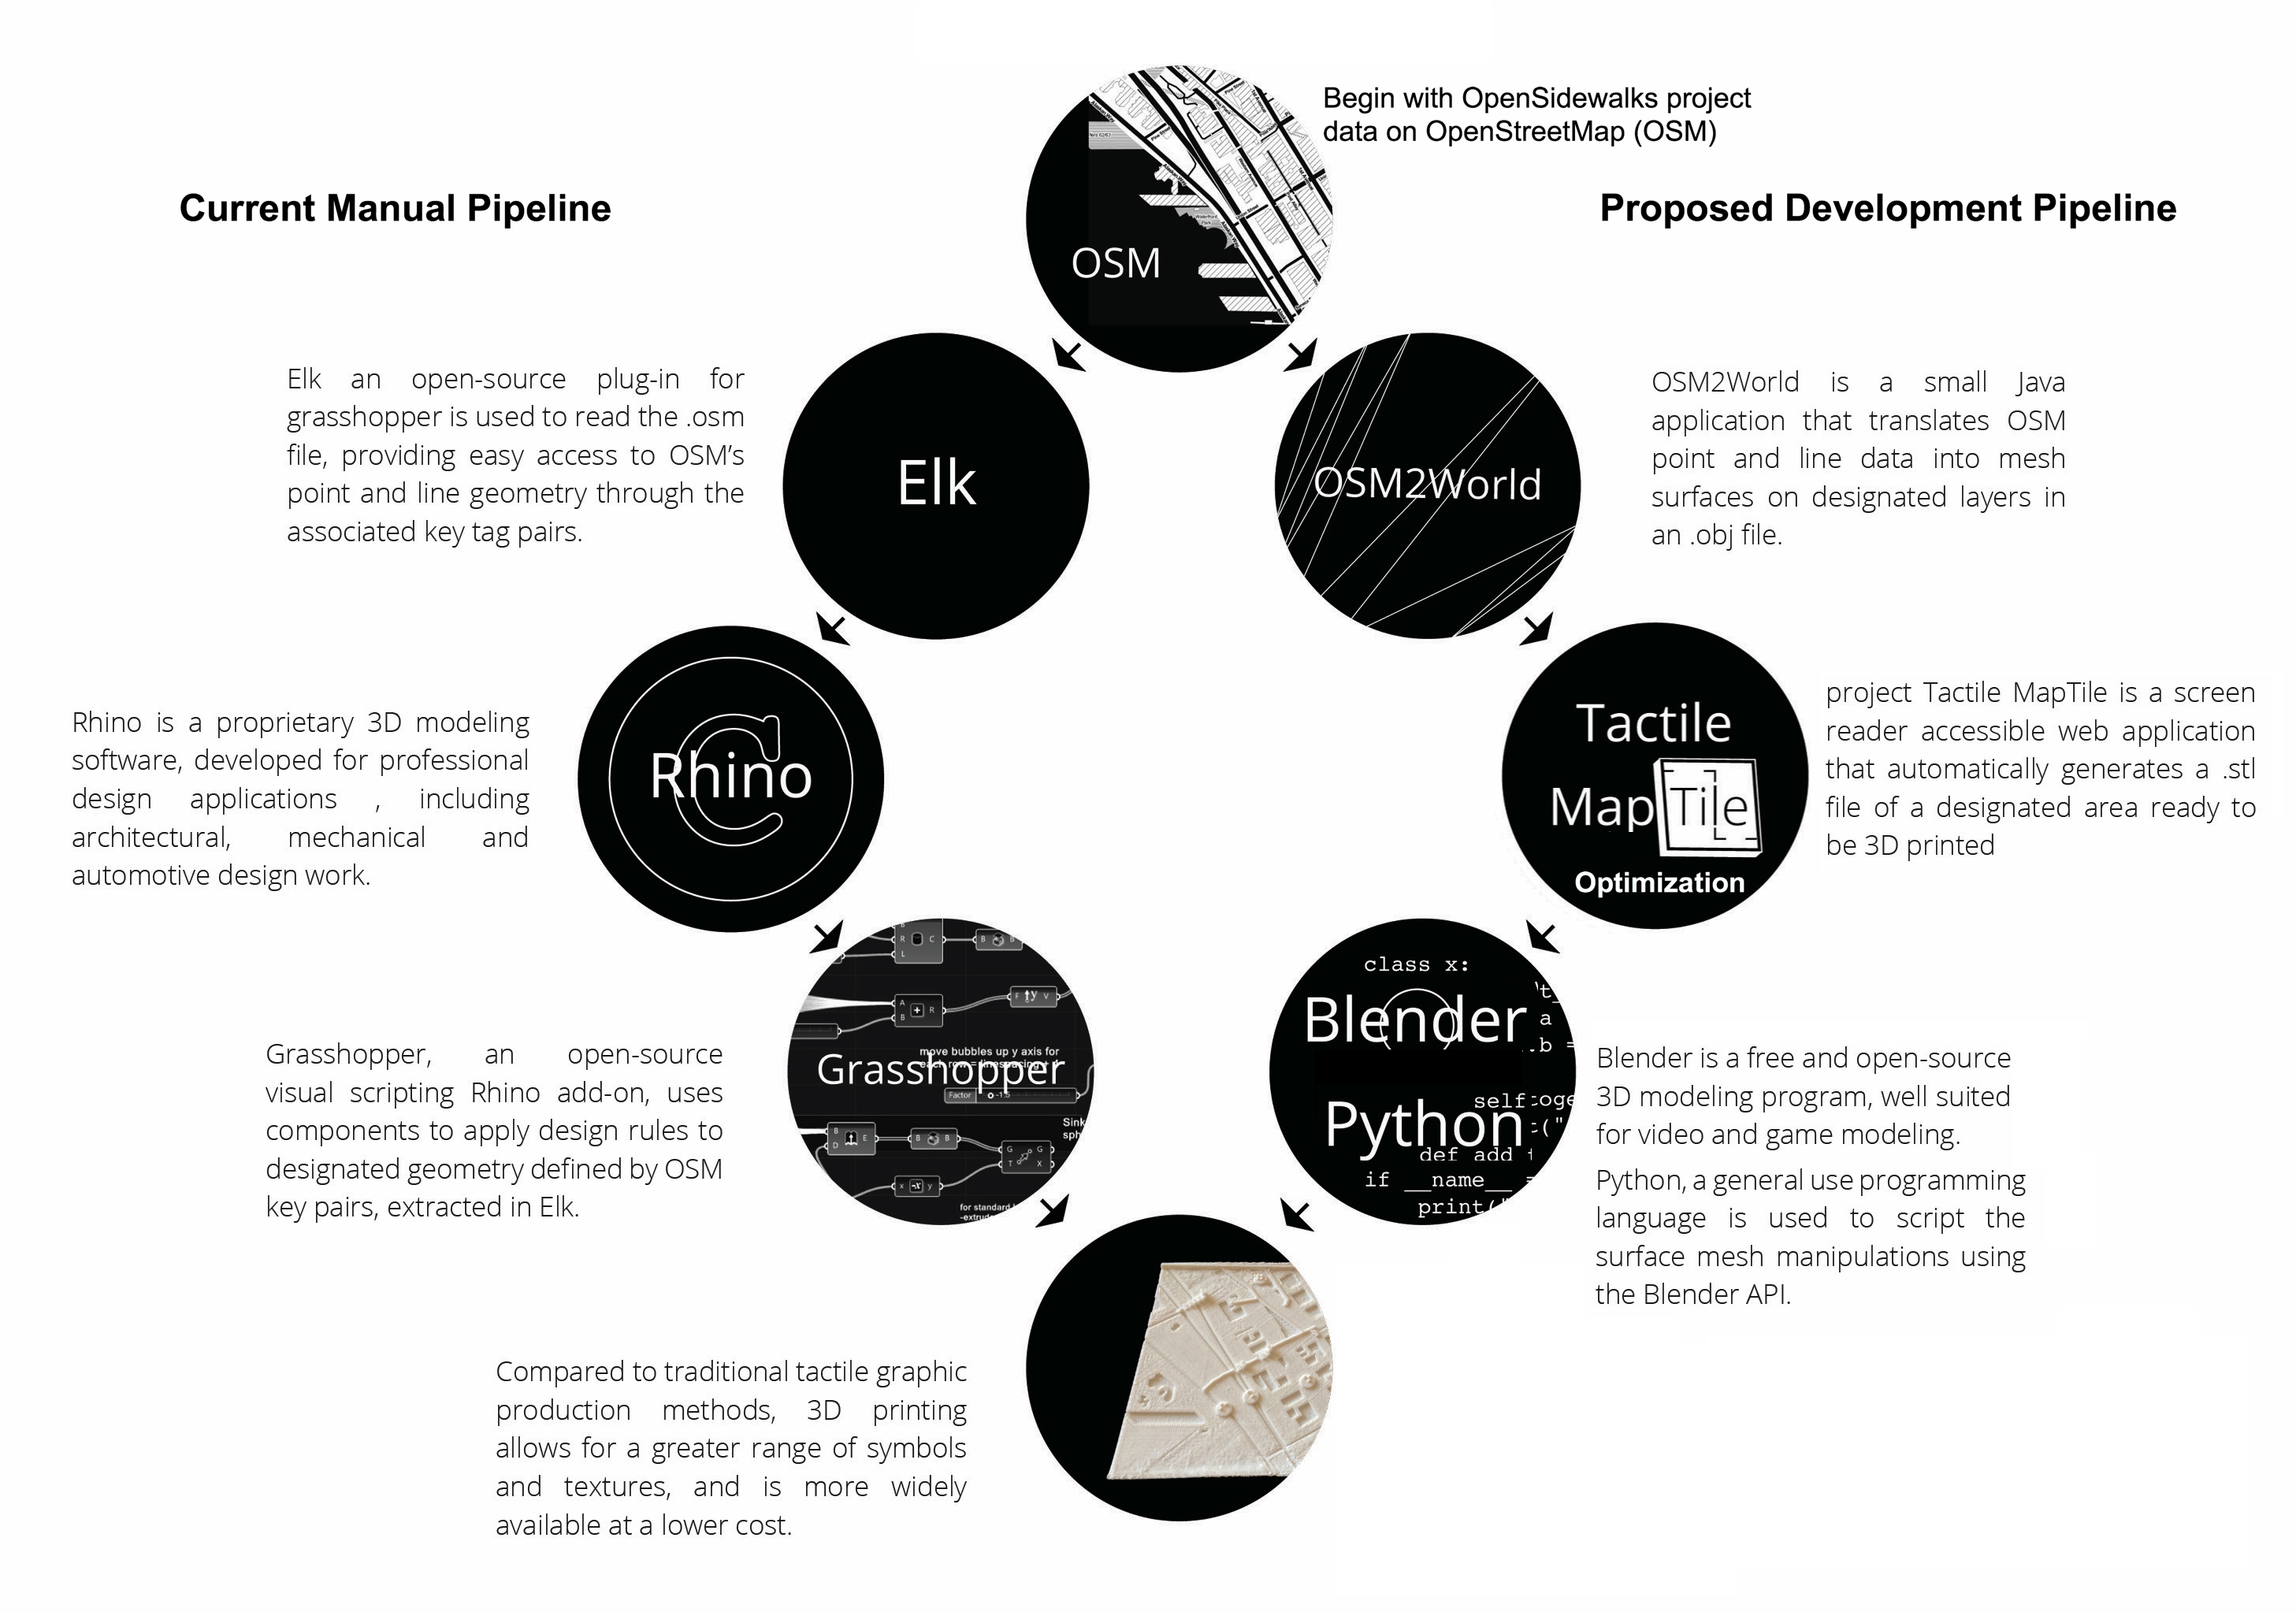
\includegraphics[width=5.5in]{pics/TactileMaptilePipeline.jpg}
    \caption{Tactile Map Tile Development Pipeline}
    \label{fig:TactileMapTileDev}
\end{figure}


\begin{comment}

\ac{ THIS SECTION IS A HODGE PODGE. NEED TO DESCRIBE: WHAT WILL BE DEVELOPED, TECHNICAL EVAL (SUCCESS METRIC) AND USABILITY EVAL (METRICS)


While tactile interactions have been studied extensively by others (\textit{e.g.}, see this review \cite{o2015designing}) as well as our team (\ac{cite ASLA 2017}), the specific design considerations for tactile maps are not as well understood, particularly for Deaf-blind individuals. In addition, no computational model that takes these variables into account exists (this is the subject of Section\ref{sec:optimize}).

to do: Megan to describe how she will create atomic semantic features to be included in the models. Also need to describe how she will test that the material composition is comfortable for the users, and how she will engage participatory design methods in figuring out the right scale, the right Braille, legend, etc., basically need to respond to the enumerated point considerations
%(C) The proposed project employs appropriate samples in tests, trials, and other development activities. (D) The proposed project conducts development activities in appropriate environment(s). (E) Input from individuals with disabilities and other key stakeholders is obtained to establish and guide proposed development activities. (F) The applicant identifies and justifies the stage(s) of development for the proposed project; and activities associated with each stage. }
\end{comment}

\subsubsection{Validation}

The following validation statements should be tested and hold true if the design goal for this development activity is met: 

The developed pipeline improves reproducibility and accessibility of map information options relative to prevailing options for travelers who are Deaf-blind.

The developed pipeline does not exceed in cost or time over prevailing services.

Here we describe our validation tests for both statements. The data elements and sources are referencing tests and data collection that will occur with our community partners. These data collection activities are described in later sections with greater detail.

\textbf{Validation Statement 1:
The developed pipeline improves reproducibility and accessibility of map information options relative to prevailing options for travelers who are Deaf-blind.}

\texttt{Performance Metrics:} Change in perception of information content and accessibility of information during a two-phased alpha and beta approach, demonstrating improvements in mental models of area, satisfaction and feedback. Also used as metrics would be survey questions designed to assess the baseline access to map information nationally via the national outreach survey instrument (described in Section \ref{test:baseline}). Additionally, responses to questions regarding the perception of accessibility and reproducibility of mapping options for individuals who are Deaf-blind will be used.

\texttt{Data Elements \& Sources:}
Early Development Baseline Survey (Section \ref{test:baseline}) and 
Surveys of User Groups: alpha and beta populations (Section \ref{test:usersurvey}).

\texttt{Analysis Procedure:}
The survey data collectively would be used to evaluate this hypothesis.  The survey responses will be aggregated according to specific metrics that capture relevant information, such as the percentage of users who feel as though the Tactile Map Tile option has (1) increased their overall access to map information, or (2) increased access to better information.  
The survey will be deployed to the identified beta user group. Since the survey will include the elderly along with younger adults — all of which will be identifiable through survey questions — we will disaggregate the analysis on separate demographic cohorts as necessary.

\textbf{Validation Statement 2:
The developed pipeline does not exceed in cost or time over prevailing services.}

\texttt{Performance Metrics:} Change in cost and time to access tactile map services with our alpha and beta populations. Also used as metrics would be survey questions designed to assess the baseline cost and time to access tactile and other map information nationally via the national outreach survey instrument (described in Section \ref{test:baseline}). 

\texttt{Data Elements \& Sources:}
Early Development Baseline Survey (Section \ref{test:baseline}) and 
User Groups: alpha and beta populations (Section \ref{test:usersurvey}). Please see test description for suggested population sample.

\texttt{Analysis Procedure:}
The survey data collectively would be used to evaluate this hypothesis.  The survey responses will be aggregated according to specific metrics that capture relevant information. No disaggregation by demographics will be used for this validation.

\begin{comment}

\textbf{usability evaluation for map scale and symbol size}
Due to 3D print bed constraints, map tiles were limited to ~8” x 5.5”. At this scale, 3 tiles are needed in order to capture an area that includes approximately 1.5 squared mile. Based on preliminary feedback from expert users, basic features of the urban pedestrian environment were legible at this scale.  Further usability testing and symbol development will be conducted during our development project in order to assert that this scale is appropriate for use as a navigational aid. In our pilot \ref{sec:pilot} case study map series was printed with slight variation in symbol style, and size on each tile for user testing. In our development project participatory process, we will increase the variations produced and exaggerate some of the detailed features to assess user preferences for map scale and symbol size under different contexts of map use.


From a research perspective, one open problem is combining tactile maps and smartphones. By embedding capacitive touch sensing capabilities in tactile maps, it is possible to provide audio feedback about the region someone is touching \cite{taylor2016customizable, rusu2010semantic,gotzelmann2016lucentmaps}. 

Finally, questions remain about the ability of tactile maps to support route finding (as opposed to orientation). For example, Gual \textit{et al.} found that standard 3D printed maps can improve memorization in route finding, but could not be used autonomously without collaborator support \cite{gual2012visual}. However, they did not explore a wide range of tactile variables to support interpretation. 


\end{comment}



\subsection{Data and Symbol Abstraction: Incorporating Critical Pedestrian Features and Standard Tactile Symbols}

This section describes development activities to incorporate into our solution the appropriate type of information with the appropriate tactile symbol representation to fit the informational requirements of for our user population. 
The development activity of incorporating dense information about footpaths and transit for travelers who are Deaf-blind is the second part of delivering tangible map design (Product 1). 
We discuss why other interfaces (like voice labels reproduced on Braille dispays) may be inferiorto 3D printed maps in mediating some of that information.

Development Goal: Use scalable, standardized methods to collect, represent and maintain open source data about pedestrian environments and use General Transit Feeds for updated information about fixed route transit.

\label{sec:mapping-data}
%(i) The extent to which the proposed project methodology is meritorious, including consideration of the extent to which: (A) The proposed project shows awareness of the state-of-the-art for current, related products. (B) The proposed project employs appropriate concepts, components, or systems to develop the new or improved product. (C) The proposed project employs appropriate samples in tests, trials, and other development activities. (D) The proposed project conducts development activities in appropriate environment(s). (E) Input from individuals with disabilities and other key stakeholders is obtained to establish and guide proposed development activities. (F) The applicant identifies and justifies the stage(s) of development for the proposed project; and activities associated with each stage. 

\subsubsection{Background and State of the Art}

Two significant factors impact how effective tactile maps are as tools for enhancing spatial understanding: what information is contained on the map and what tactile symbols are used. 

\textbf{What tactile symbols to use}
The majority of tactile mapmakers are orientation and mobility specialists, typically employed through special education programs
\cite{lobben2012tactile}, \ac{Rowell and Ungar 2003c}. While this implies they are experts in the needs and limitations of people with visual impairments, formal training in cartographic design is limited. There have been some efforts to codify and standardize symbology for tactile maps, however the work has been scattered and there does not yet seem to be a consensus in adoption. Additionally, as illustrated by the annals of graphic map history, there is no guarantee that standardization will result in good maps. Tools produced by mediators limit the agency afforded by the opportunity to dictate one’s own priorities and are susceptible to biases in terms of what information is presented and how that is prioritized. 

In 2012 researchers from the University of Oregon published a comprehensive set of tactile map graphic symbols.  This standard was adopted by the Braille Authority of North America (BANA), to be distributed in their tactile graphics publication
\cite{lobben2012tactile}. However, to date, the only documents available on the BANA’s website predate Lobben and Lawrence’s publication, and thus do not include these proposed standards. In our development, we intend to use this as our reference tactile symbol standard.

\textbf{What information to include}

We consider what information ought to be represented in a tactile map that needs to include the most pertinent information for Deaf-blind individuals to travel in the street environment. Sidewalks are at the heart of traveling through urban centers with low or no vision, and sidewalks support transitions between nearly all other travel options. While having accessible infrastructure such as Tactile Accessible Pedestrian Signals (APS that include a tactile plate rather than only auditory cues) is clearly necessary, knowing of the location of infrastructure (and obstacles) can be equally so. Though we cannot make all sidewalks accessible overnight, foreknowledge of avoidable obstacles aids independent and empowered pedestrian travel.

However, with typical map data (from both proprietary and open sources) it is not currently possible to give a Deaf-blind person an updated tactile map representation that is a relevant, reliable, current record of pedestrian paths accessible to them to or from any location due to a lack of data about the walking environment.  
There are no major digital mapping services to date with a comprehensive sidewalk dataset (\ac{Apple 2019 , Microsoft  2019, Google 2019, OpenStreetMap 2019}). Many cities have made attempts at collecting this data, willingly or otherwise, but disparate efforts, risk being outdated before they begin and often are done in such an imprecise manner that significant clean up needs to be done before the data can be utilized for routing, or other applications that require a finer granularity of data \ac{(Bolten et al. 2016)}. 

Our preliminary studies showed us that this informational gap forces Deaf-blind individuals to risk exploring unverified routes that may strand them in dangerous situations, or abandon independent travel to unknown locations altogether. Furthermore, due to the lack of data and mechanisms, it is not currently possible to systematically ascertain what obstacles exist on a given path, and therefore this social inequality is largely hidden from public view.

\subsubsection{Previous Development}

The OpenSidewalks Project is a data project for the standardized detailed description and appropriate data collection of sidewalk infrastructure.
OpenSidewalks represents a collaboration of data scientists, tool developers, urban specialists, open data communities, educational software specialists, and local advocacy groups, all of whom work to promote equitable and resilient accessible cities.
OpenSidewalks is led by the Taskar Center for Accessible Technology (TCAT) at the University of Washington, who is a project partner.

Our prior work in the OpenSidewalks project defined a data standard for describing the pedestrian environment and the pedestrian network. OpenSidewalks promotes equity in pedestrian routes by making sidewalks first-class members of an open data transportation network \cite{bolten2017}. Collecting open sidewalk information supports a variety of use cases and downstream activities, including addressing the informational gap for pedestrians of all abilities, automated trip planning customized to individual abilities, and furnishing rich analytic tools for data-driven urban planning. 

In order to facilitate the end goal, the OpenSidewalks project focused on employing open source, crowd contributed, geospatial data from OpenStreetMap (OSM). OpenStreetMap was chosen for its extensive global coverage and easily extendable data schema. This platform allows for the project to easily pull from a large existing data pool, while also making it simple enough to fill in informational gaps as they pertain to pedestrians. For inclusion of updated transit data, OSM is also an appropriate platform choice since it is designed to include support for updated transportation data from fixed-route services (GTFS feeds) \cite{OpenStreetMap}.

There are many aspects of the pedestrian environment that we consider for inclusion in pre-optimized tangible map tiles for people who are Deaf-blind.  Based on our pilot focus groups and informational interviews, we incorporated \textit{surfaces}, \textit{topography} and \textit{street interfaces} into our own published data standard described by OpenSidewalks; these critical features promote wayfinding, mobility and safety for people with a range of visual capacities. Figure \ref{fig:DataFeatures} demonstrate the features of a surface that were evaluated for inclusion in the maps. 

\begin{figure}
    \centering
    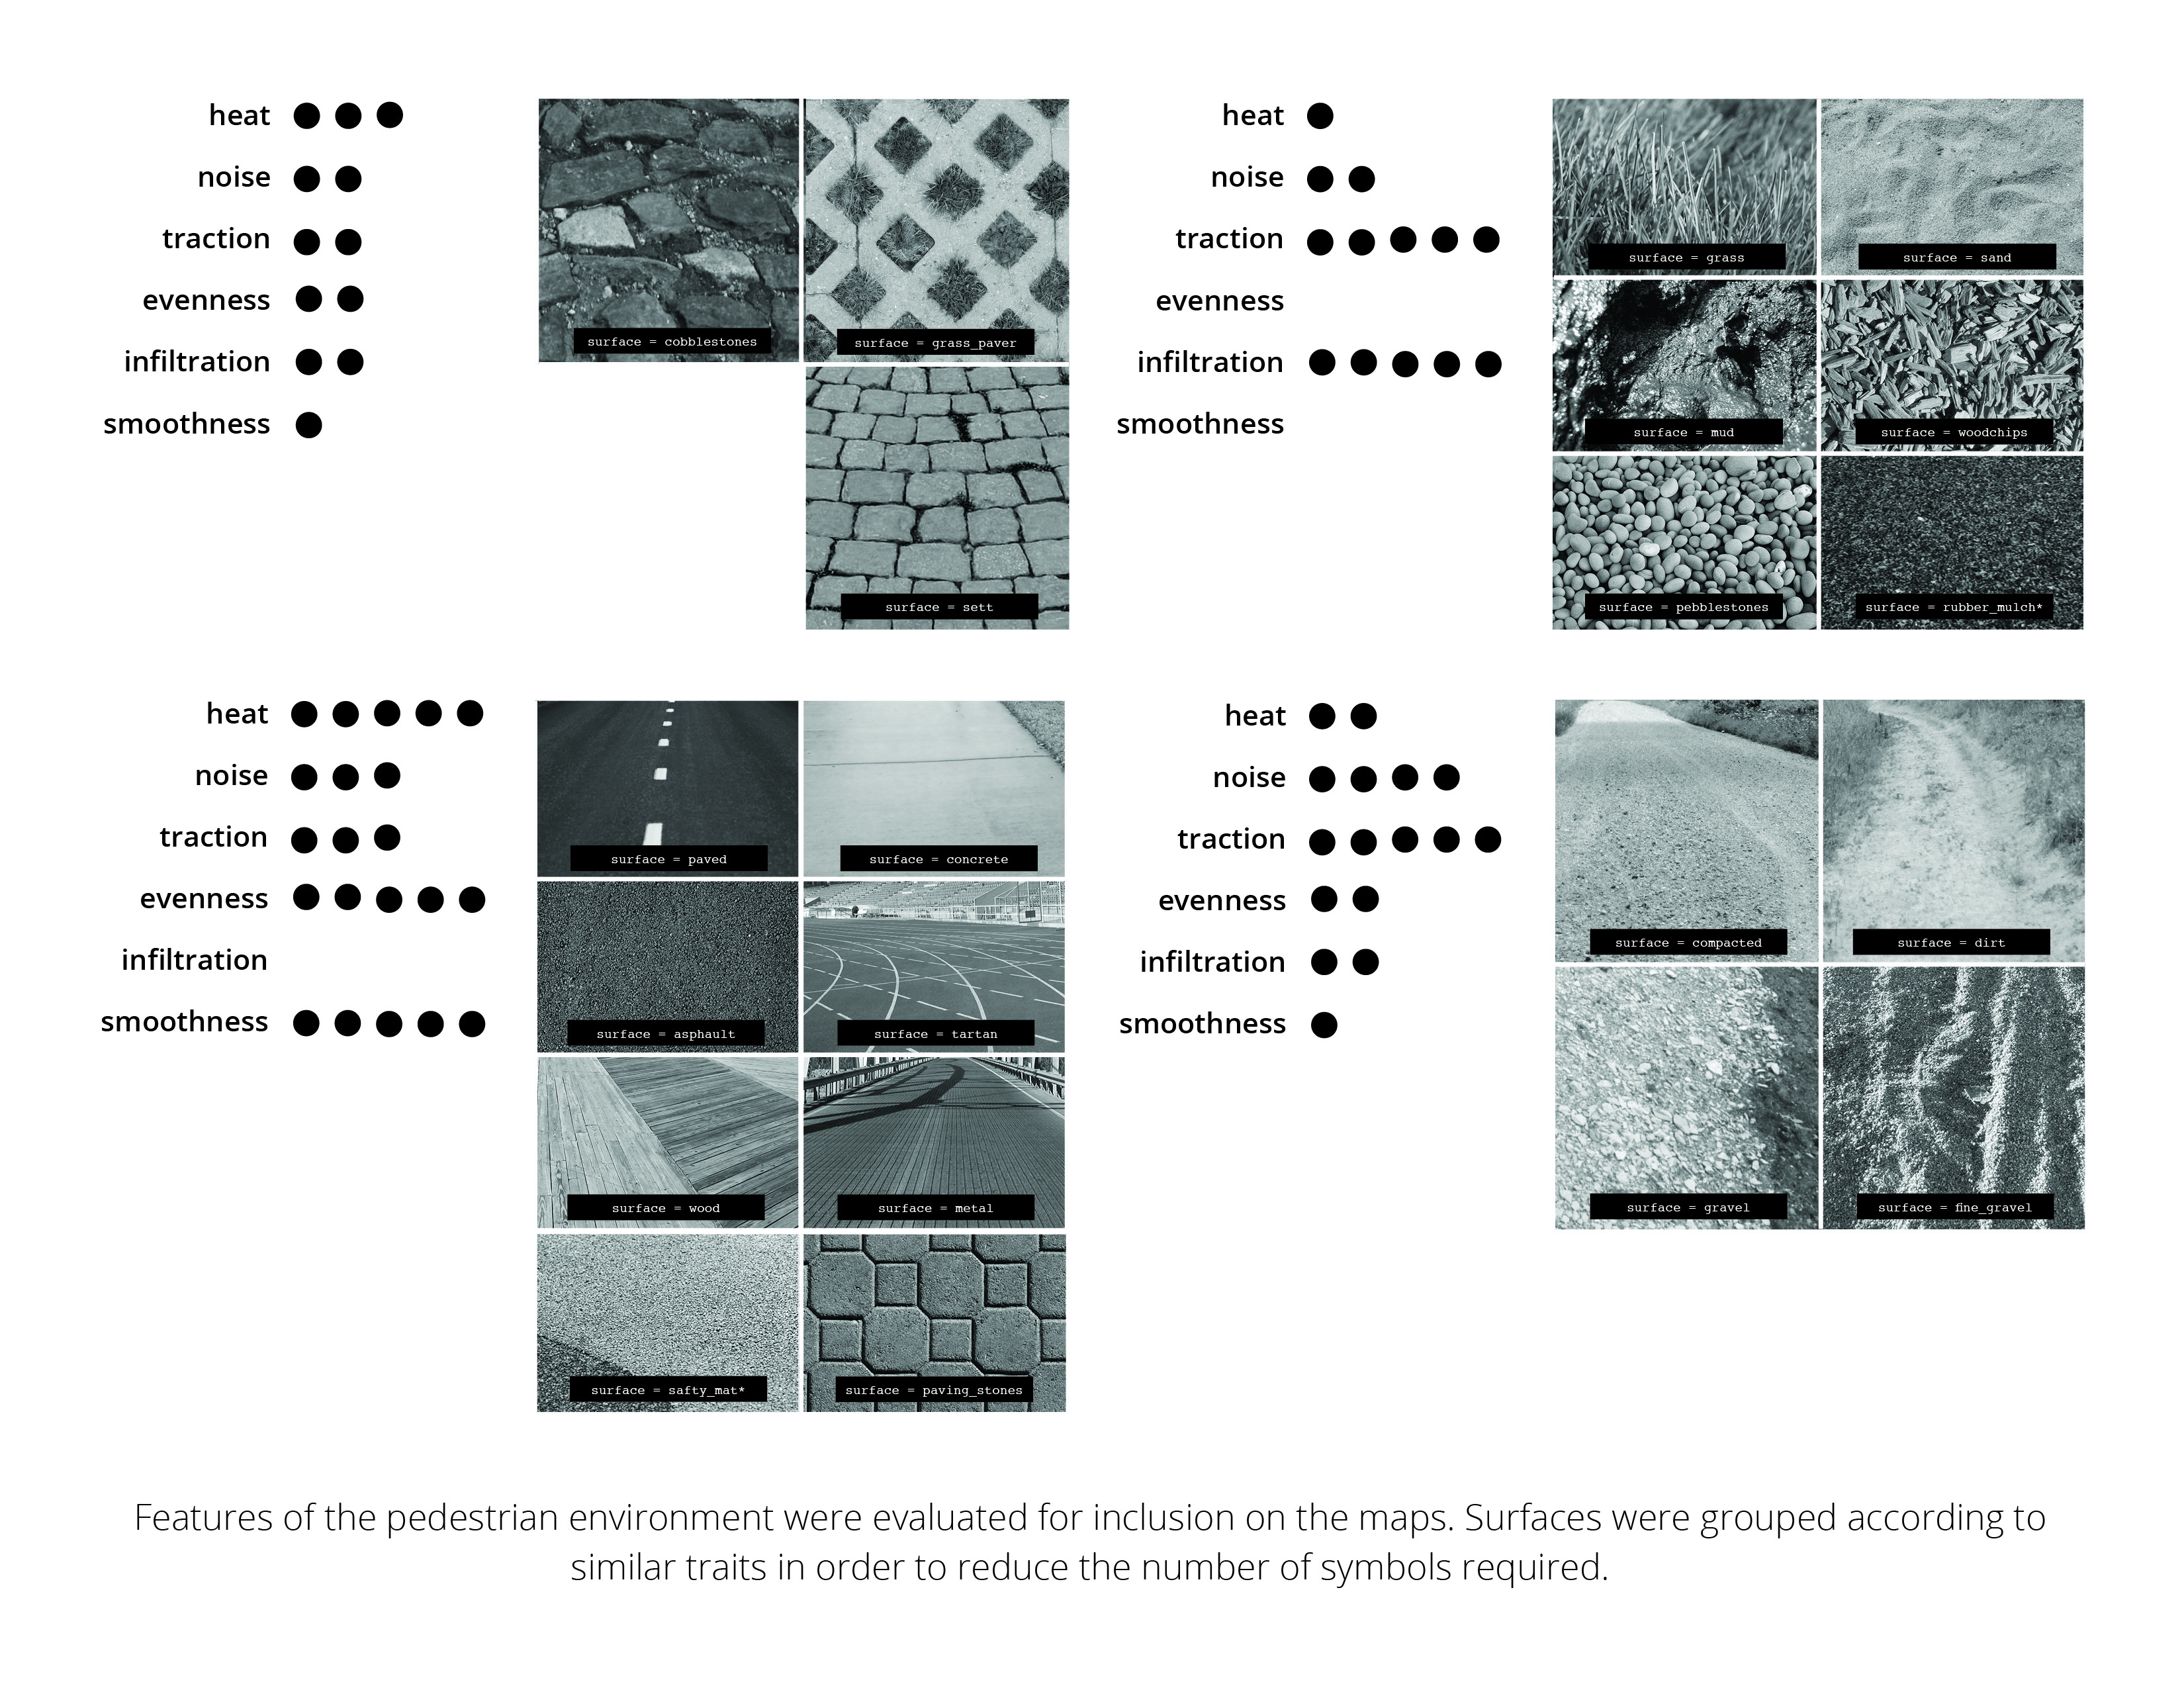
\includegraphics[width=5in]{pics/SidewalkFeatures.jpg}
    \caption{Features of footpath surfaces included in the OpenSidewalks data standard, for inclusion in our tactile maps}
    \label{fig:DataFeatures}
\end{figure}

Appendix \ref{sec:standarddata} includes an overview of features the OpenSidewalks data project collects pertinent to blind, low vision and Deaf-blind pedestrians. As requisite features of any pedestrian environment, surfaces are first explored, followed by topography, which is nearly as ubiquitous.  Street interfaces, while occupying less space in a pedestrian environment, arguably have the greatest impact on pedestrian safety and well-being and are the third feature set considered. 


\subsubsection{Proposed Development}
Only some of the surface features we discuss have been studied in relationship to the experience of visually impaired pedestrians (Secchi, Lauria, and Cellai 2017). 

In this development task, we plan to fully collect all the cartographic features of the OpenSidewalks standards in two pilot areas. This will 
support the development and testing of our Proof of Product application.
We will use the data in the creation of the tactile maps to enable both testing the optimization algorithm we develop (Section \ref{sec:optimize}) and appropriate environments for field studies (Section \ref{test:fieldstudies}). We will be able to better answer several open questions remaining in understanding the use of the standards towards fabricating Tactile Maps with pilot zones in very different environments:
\begin{description}
\item[Downtown Seattle by City Hall] This area contains a significant volume of Seattle's fixed-route bus lines and lightRail transit, including two undergraound stations. The Downtown Seattle Zone will be the testing ground for many important use cases including servicing 
users who take transit to travel to or from a downtown core, with a highly complex geographical topology (many hills) and transit and pedestrian network.
\item[The University of Washington LightRail Station] is a transit transfer center and a park‐and‐ride, along with a hub for hospitals and patient care facilities. The University of Washington Stations 
Zone will be the testing ground for the transfer center use case: a traveler needs to transfer from one transit route to another and must locate the appropriate bus bays within the transit center to complete his or her trip.
\end{description}

\begin{comment}
push this to validation

First, we need to provide a prioritization of the cartographic features from OpenSidewalks as they pertain  ascertain which of the pedestrian cartographic features from OpenSidewalks should be prioritized in tactile maps given that not all could be equally weighted \cite{haberling2008proposed}.
Second, the features we describe may not be appropriate for all map scales or travel purposes.   
Third, our previous tests did not include field testing. 
We ought to offer different weighting for different map purpose (for example, bus stops are not as highly prioritized when users request a map for local exploration, whereas bus stops and their amenities need to be highlighted when a map is requested for a specific transit trip).

\end{comment}



\subsubsection{Validation}

The following validation statements should be tested and hold true if the design goal for this development activity is met: 

Detailed sidewalk layer data is available for all streets in the pilot regions.

Updated transit feed data is available for all streets in the pilot regions.

Here we describe our validation tests for both statements. The data elements and sources are referencing tests and data collection that will occur with our community partners. These data collection activities are described in later sections with greater detail.

\textbf{Validation Statement 1:
Detailed sidewalk layer data is available for all streets in the pilot regions.}

\texttt{Performance Metrics:} 

\texttt{Data Elements \& Sources:}

\texttt{Analysis Procedure:}

\textbf{Validation Statement 2:
Updated transit feed data is available for all streets in the pilot regions.}


\texttt{Performance Metrics:} 

\texttt{Data Elements \& Sources:}

\texttt{Analysis Procedure:}


\subsection{Optimization: Best Utilization of Constrained Tactile Space} 

This section describes development activities to optimize the tactile map content so as to balance information richness with tactile usability. For our maps to be used in practice, we must utilize optimization algorithms to create maps that are information-rich, but make appropriate use and density of tactile features to afford maximum usability.
In addition, the optimization schema must be parametrizable in order to best accommodate the user’s requirements about the area of travel, type of travel, and other travel needs and preferences.
\label{sec:optimize}

\subsubsection{Background and State of the Art}

Route planning requires information that may be specific to the person creating a map. For example, Google Maps routes pedestrian directions from University Street Station on Second Avenue to Seattle City Hall on Fifth Avenue up Seneca Street, which has a steep 10 percent grade that is problematic for people in wheelchairs or with certain injuries or health conditions.
%SK:  how about older people?  That's not a "health condition" to me :).
%In contrast, AccessMap routes people two blocks north to Pike Street, which has a much gentler grade of less than 2 percent.
%For such people, it is important to ensure that a map clearly indicates slope. For those concerned about safety, however, it might be more important to show whether a guard rail is present near a particularly busy street, whether a sidewalk is wide or narrow near a busy street, or whether an alternative pedestrian route connects their sidewalk to a pedestrian footpath removed from the road. 
%For accessibility, 
users have varied needs.  A powered wheelchair user may need to know the location of curb ramps to navigate an intersection. A blind user may want to actively avoid certain types of curb ramps (such as those pointing to the center of an intersection). These different informational requirements present a particularly difficult situation to resolve without a detailed description of the available paths, how they are connected, and particular attributes (like curb ramps and their locations) \cite{bolten2017}. Furthermore, it is not possible to represent every possible piece of important information on any map. In particular, the amount of information that can be represented is further reduced in a tactile map. 
%SK:  Explain reason for preceding statement.

%SK.  Start discussion here.
\textit{Optimization} algorithms makes tactile maps accessible and actionable.  Here, we describe both: (1) optimizations that balance information richness with tactile usability, and (2) optimization cost functions that allow customization by Deaf-blind users of varied aspects of their travel experience.
%SK:  Now define optimization and what it does.

\jm{does this go in introduction instead?. also more about what optimization is/does A: I think that's where we were going before and it blew up the introduction. I think it's important to highlight here how optimization can make these maps actionable.}

\subsubsection{Previous Development: Optimization Approach}
Maps use many renditions to represent various forms of information. A  rendition could be a type of icon, or a colored line. Each rendition can represent only one class of information in a map. For example, a circular icon could note an accessible intersection, or a guide-dog friendly coffee shop, but it would be confusing if it represented both. Not all forms of information are compatible with all renditions. You cannot represent a road with just a circular icon. 
%The binary value stating if a a piece of information (a.k.a., a datum), $d$, is compatible with an rendition, $r$, is denoted $c_{rd} \in \{0,1\}$. If the datum is then assigned to a compatible rendition, this is denoted with the binary value: $x_{rd}\in \{0,1\}$

Our goal is to assign the most relevant pieces of information to the most useful renditions while maximizing the amount of information we present.  To do this, we need a model that describes what the most relevant information is.

%The zero-one linear program is formulated as follows:
%\begin{equation*}
%\textrm{ argMax }
%\sum_{i=1}^{|R|}
%\sum_{j=1}^{|D|}
%\alpha(r_i, d_j) x_{ij}
%\end{equation*}

%\begin{subnumcases}{
%\textrm{ s.t. } 
%}
%   \forall_{i \leq |R|} \forall_{j \leq |D|} r_{ij} x_{ij} \leq r_{ij} \label{data_rendition_compatability}\\
%   \forall_{i\leq|R|} \sum_{j\leq|D|} x_{ij} = 1 \label{rendition_Cap} \\
%\forall_{j\leq|D|} \sum_{i\leq|R|} x_{ij} \leq 1  \label{unary_data}\\
%\sum_{i\leq|R|} \sum_{j\leq|D|} x_{ij} = %\min(|R|, |D|) \label{complete_fill}
%\end{subnumcases}

%\item[Weighting Information-Rendition Pairings]
Specifically, when deciding how (or whether) to render a piece of information, we must consider three features with the acronym (CIA): the rendition's communicative ability (C), the data's importance (I), and the attentive cost (A).
%SK: Will readers know what "attentive cost" means? You use this interchangeably with "attention cost."  I changed all refs to the former for consistency.
We combine these by subtracting the attentive cost ($A$)  from the benefits ($C*I$): 
\begin{equation}
\label{eq::CIA}
\alpha(r_i, d_j) = C(r_i, d_j)*I(d_j)-A(r_i, d_j)
\end{equation}

\begin{description}
\item[Communicative Ability]
Communicative Ability, $C(r,d)$, is the measure of how well a rendition, $r$, communicates a specific type of information, $d$.
%A high level measure of this is already accounted for in the hard constraints of the linear program: if a rendition is incompatible (\ie incapable of communicating a class of information) constraint \ref{data_rendition_compatability} will not be met and the pairing will not be accepted. But our model must support more nuanced expressions of information communication. 
%For instance, there may be many types of renditions that label a coordinate on a map, but each are subject to certain limitations. 
For example, the number of parallel roads that can be represented in a space depends on the width of the lines representing the roads; denser road networks require thinner lines, while sparse networks could make use of more distinguishable, thicker lines. Further, certain attributes of a rendition may be more or less desirable to a specific user, such as the preference for braille or embossed text. 
%In our system, all renditions have a set of attributes, $a \in A_r$, (\eg uses braille, uses raised edges vs uses indented edges). Similarly, users profiles, $U$, and classes of information, $d$, have a set of preferred attributes, $\hat{A}_U,\hat{A}_d$ and weights on those preferred attributes $\beta_a$. 
More formally, the communicative ability of an information-rendition pairing is the weighted sum of the intersection of a rendition's attributes, an information class's preferred attributes, and a user's preferred attributes. 
\begin{equation}
\label{eq::communicability}
C(r,d,U) = \sum_{a\in A_r \cap \hat{A}_d}(\beta_a) +  \sum _{a\in A_r \cap \hat{A}_U}(\beta_a)
\end{equation}
%Attributes can be expressed in many ways, and determining the intersection of a rendition's attributes and preferred attributes is managed through a series of adapter interfaces. For instance, one interface is a Braille-compliant rendition, which requires the rendition to generate related text in braille. A user profile and information maintains a list of relevant adapters (\ie the preferred attributes) mapped to the preferential weight and any parameters of that preference. An example parameter is a preference for lines no thicker than 2 mm or no shorter than 1mm. These parameters are applied to the rendition through the adapter. 

\item[Information Importance]
%Information importance is the simplest measure of an Information-Rendition Pairing and it is central to the adaptive design paradigm our system represents. 
Users know what information is important to them. They know the accessibility features and challenges that affect them most, and what points of interest are most relevant to them. %For this measure, we simply 
Thus, we ask users to rank information. %, the higher the ranking, $I(d_j)$, of a class of information, the higher the weight. If the information is useless or irrelevant to the user the ranking is set to zero which intern makes the weight, $\alpha$, on all rendition pairings with this information zero or less, guaranteeing that the information will not be presented. For efficiency reasons, information classes that are marked as having no importance are excluded from linear program a priori. 
We can pre-populate this with default rankings based on a survey of typical user preferences. 

\item[Attentive Cost]
The attentive cost of a rendition measures how distracting it is to gather information from it. For example, if a user were using a rendition of a road network to navigate the map in search of a target, say their favorite coffee shop,  the longer it takes to find the target the more information they must keep track of (\textit{e.g.,} where they started, what turns they made, what landmarks they noticed). Tracking all of this information carries an attentive cost that would otherwise be spent on the primary search task.

A key problem here is that when the map is being constructed and the attentive cost weight is needed, we do not know what the user's target(s) will be, where they will start their search, or what other information is presented that may help or hinder the search task. To address this, we will use a Monte-Carlo simulation of user behavior based on our experimental work.\jm{megan: reference for monte carlo?} %The presentation of that information is, in fact, our goal. Given this level of uncertainty, we use a Monte-Carlo simulation to estimate the average \textit{time} it takes for the user to perform a search given a rendition-information pairing. The probability distribution used to generate this Monte-Carlo simulation is derived from a Markov-chain state model representing the actions a user can take when he or she encounters portions of a rendition. 
%\begin{figure}
%\label{fig::exampleStates}%
%	\begin{tikzpicture}
%        % Add the states
%        \node[state] at (0, 0) (o) {Off Road};
%        \node[state] at (4, 0) (r) {On Road};
%        \node[state] at (2, 4) (i) {Intersection};

%        \draw[every loop]
 %       	(i) edge[loop left] node {} (i)
%        	(i) edge[bend right=20] node %{} (r)
%            (r) edge[bend right=20] node {} (i)
%            (i) edge[bend right=20] node {} (o)
%            (o) edge[bend right=20] node {} (i)
%            (o) edge[loop left] node {} (o)
%            (r) edge[bend right=20] node {} (o)
%            (o) edge[bend right=20] node {} (r)
%            (r) edge[loop right=20] node {} (r);
%    \end{tikzpicture}
%\caption{Example of states of navigating a road network}
%\end{figure}
\end{description}

%Suppose that a user is navigating a rendition of a road network. There are three basic states of the action: (1) moving a finger along the road, (2) encountering an intersection of roads, and (3) moving a finger along the new road. Which particular state the user is in depends on the specific roads paired to the rendition, and their likelihood of moving from one state to another depends on both the particular road network (the information) and the rendition. For example, when the user encounters an intersection, he or she is very likely to continue onto a new road (\eg changing from the Intersection to On-Road state), but which road depends on many factors. Generally, the user is more likely to move in the same direction and increasingly less likely to turn all the way around. If the rendition presents very thin roads, the user is more likely to travel in a direction that they don't feel the roads any more, moving into the "Off-Road" state. We model the probability of this state change by selecting a random angle between $-\pi$ and $\pi$ from a normal distribution with a mean direction of 0 (no change in direction from the approaching road). If the user travels in that direction but could still feel a road (based on the width of the finger and thickness of the rendition), then the angle will be modified to continue along that road, otherwise they will move randomly in that general direction off-road until they find a new road to follow.  

%Each state change in the Markov-chain takes about step of one finger width, and we use a state change as a unit of time. For each simulation in the Monte-Carlo model, the user takes a "walk" across the map starting at a random point and moving towards a target. The starting points and targets are selected from a probability distribution where areas denser with information are more likely to be selected. The Markov-chain determines the walk that they take. We count the number of steps in the walk it takes to find the target given the rendition and information. The average number of steps over many models is our attention cost, meaning the more difficult (the longer it takes) it is to find information using a rendition-information pairing, the greater the attention cost and the poorer the pairing. 

%In terms of implementation, each rendition, $R$, has a set of states $S_R$. The probability of entering a state, $s_i\in S_R$, is dependent on the data, $D$, paired to $R$ and the state it is entering from, $s_{i-1}$: $P(s_i | D, s_{i-1})$, A walk over the map, $W$, starts from a starting point/state $s_1$ and we randomly change the state based on the probability distribution of all possible next-states. With each state we move the finger, $f$, a one finger width, $w_f$ in the direction dictated by the current state. The attention cost of a walk, $A(W)$, is the number of states need to get the point $f$ within $w_f$ of the target point $t$.The attention cost of a pairing, $A(R,D)$ is equal to the average attention cost of all of $N$ simulated walks.

%\begin{equation}
%W \subset S_R | s_1...s_{|W|}
%\end{equation}
%\begin{equation}
%A(W) = |W|
%\end{equation}
%\begin{equation}
%A(R,D) = \frac{\sum_{i=1...N} A(W_i)}{N}
%\end{equation}

\subsubsection{Proposed Development}

An optimization algorithm can use this information to decide on the optimal map. In optimization terms, $C*I-A$ is an \textit{objective function}, which can calculate a score for a possible map. Off-the-shelf algorithms can solve for the best solution (map in our case). For this problem, we can then  formulate the optimization as a zero-one linear program interpretation based on the Generalized Assignment Problem
\cite{kuhn1955hungarian}. 

\subsubsection{Validation}
\ac{JM: need your input here}
\ac{ make sure to include tests for both adequate balance for legibility and feature richness as well as tests for parametrization }

The following validation statements should be tested and hold true if the design goal for this development activity is met: 

The resulting tangible map depictions and choices will be valid.

\ac{this is just an example of a usability validation:}
When routing and choosing map features for no-vision pedestrians, the optimization algorithm favors streets with sidewalks and lower environmental stress (e.g., lower speed limits and traffic volume).

Here we describe our validation tests for both statements. The data elements and sources are referencing tests and data collection that will occur with our community partners. These data collection activities are described in later sections with greater detail.

\textbf{Validation Statement 1:
The resulting tangible map depictions and choices will be valid.}

\texttt{Performance Metrics:} 

\texttt{Data Elements \& Sources:}

\texttt{Analysis Procedure:}

\textbf{Validation Statement 2:
When routing and choosing map features for no-vision pedestrians, the optimization algorithm favors streets with sidewalks and lower environmental stress (e.g., lower speed limits and traffic volume).
}


\texttt{Performance Metrics:} 

\texttt{Data Elements \& Sources:}

\texttt{Analysis Procedure:}

\subsection{Integration: Providing Seamless Accessible Web Interface}
This section describes development activities for service integration into our popular AccessMap app to address, monitor, and respond to personalized transportation needs of our users.
\ac{TODO: separate the OpenSidewalks from AccessMap integration}
\label{sec:accessmap-integration}
%jen: repeats words in the bcakground section Tactile maps are not new to the cartographic record. Their value in facilitating orientation and navigation for the low vision and blind communities has been well established. However, their scope and availability has been greatly limited in the past by high production costs and limited interest from fields traditionally invested in map making and design. 

% same These maps have been designed as tools that enhance spatial understanding for people within a large range of visual capacities.  They abstract nonvisual cues from the pedestrian environment and consider circumstances that influence a full spectrum of experience. 

\subsubsection{Background and State of the Art}

\begin{comment}
I believe this is used somewhere else. Need to pull in.

Independent navigation is essential for autonomy and community participation in urban centers. 
Navigation solutions for both sighted and blind individuals fall into two important categories -- turn by turn directions, and maps. 
A common solution for Blind navigators is GPS programs that provide turn by turn directions. We tested the three blindness-aware GPS navigation mobile apps recommended by the American Foundation for the Blind: "Nearby Explorer", "The Seeing Eye GPS App", and "BlindSquare", and none offered a simultaneously sparse and informative solutions when used in conjunction with a portable Braille reader \cite{AFBBlindnessNavApps}, often because it is difficult to consume a lot of information portably with Braille readers on the go, and not all the information was equally relevant. 

\end{comment}


\subsubsection{Previous Development}
\label{sec:prev-devel-access}
The Taskar Center has two other relevant projects aiming to improve access to mobility and transportation for individuals with disabilities. The Taskar Center's overarching goal is 
to develop seamless regular-commute transportation customized assistance system that integrates multiple sources of current and critically relevant travel information.

This project build on AccessMaps, which itself depends on data from OpenSidewalks. As we will show, \jm{key points for extending accessmaps}




AccessMaps is \jm{Anat fill in introduction}.
Figure~\ref{fig:accessmap} shows the current version of the system in use. 

\begin{figure}
    \centering
    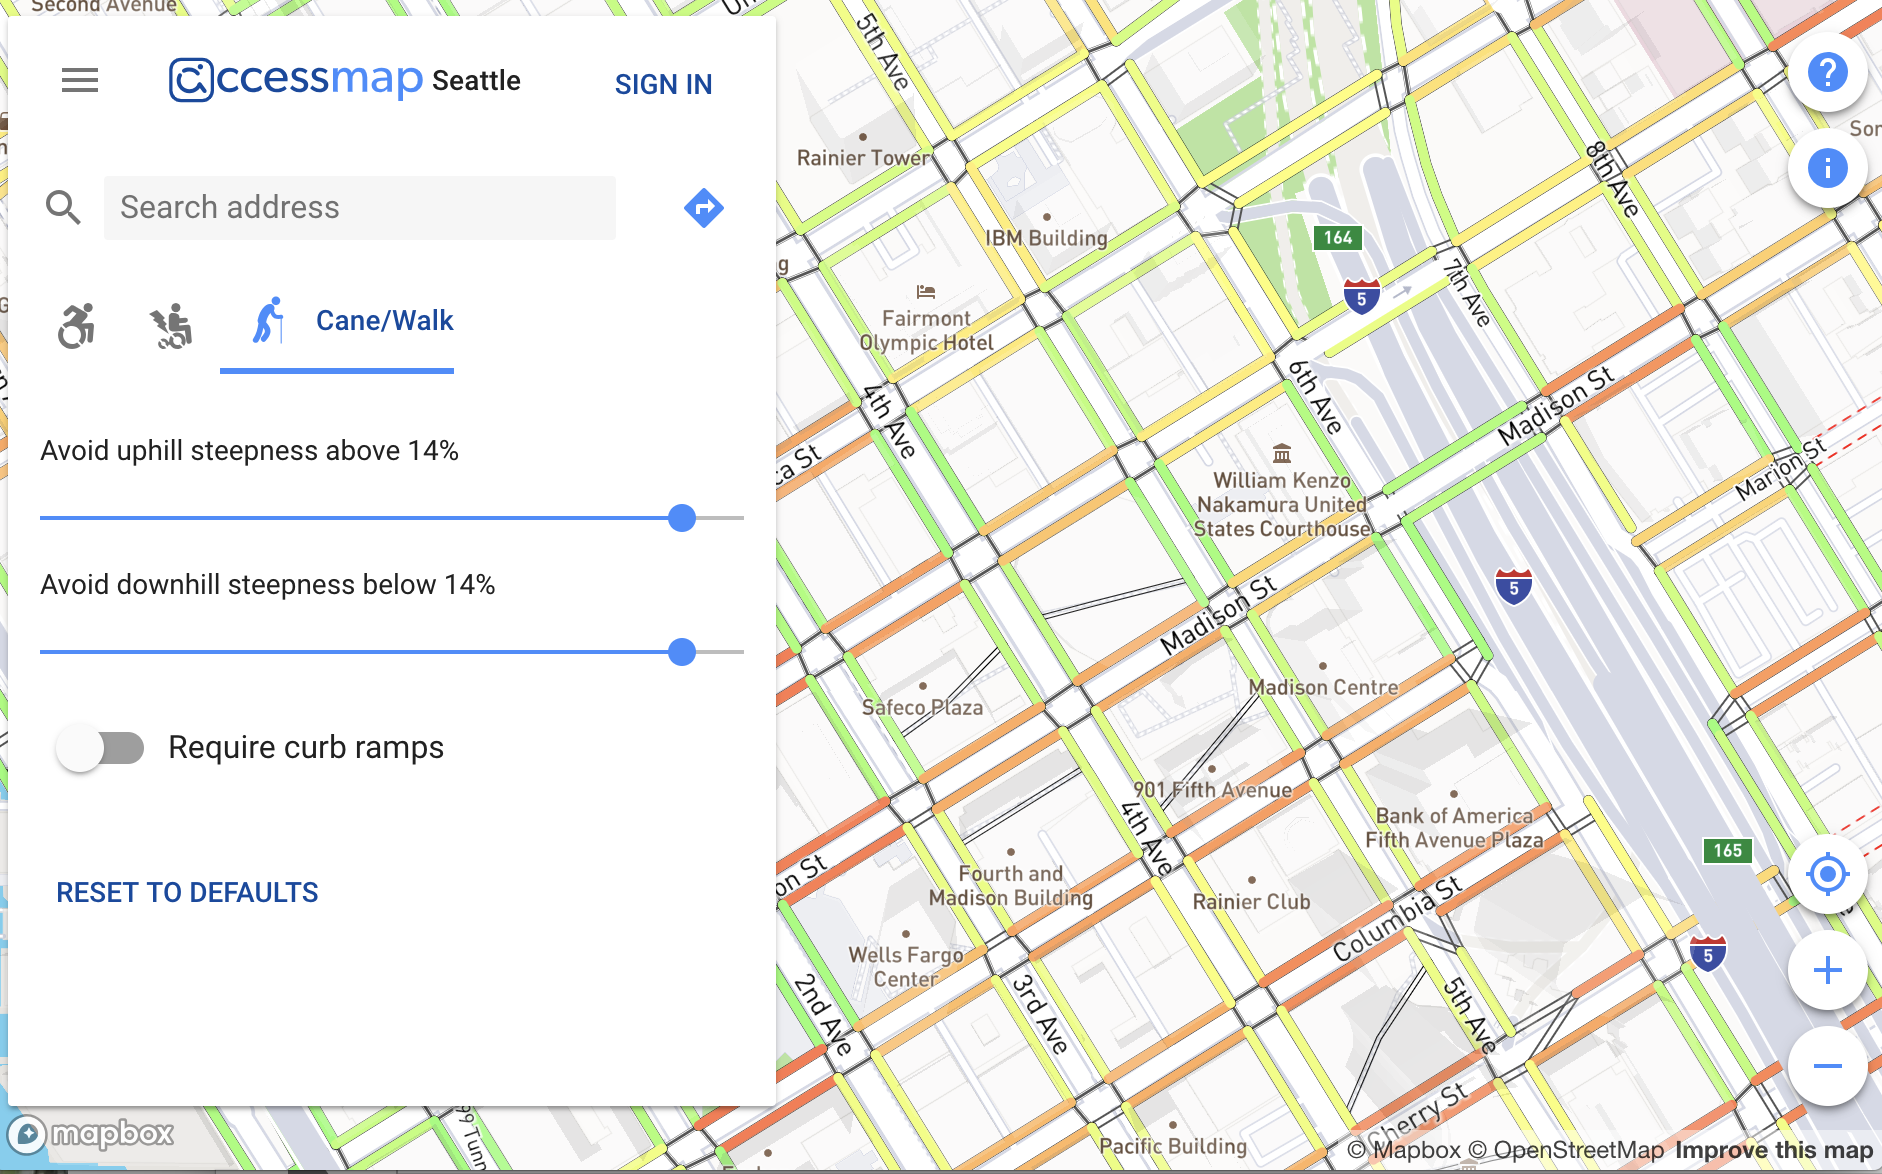
\includegraphics[width=5in]{pics/accessmap.png}
    \caption{AccessMap Screen Shot}
    \label{fig:accessmap}
\end{figure}

AccessMap currently can produce parametrically designed maps that always show the most up to data open data (derived from OpenSidewalks) about a region. 

\subsubsection{Proposed Development}

Operating hand-in-hand with AccessMap and OpenSidewalks (two projects discussed below), the goal of our work is to extend AccessMap to support users to automatically generate a custom 3D map model of any given area.  That model could then be printed at home, brought to a local library, or sent to a 3D printing service for relatively quick and inexpensive map production.  Beyond customizable map locations, ultimately the application would allow users to specify different scales and map features that are important to them.  

We will base our tactile design features on the comprehensive set of tactile map graphic symbols adopted by Braille Authority of North America (BANA) as created by (\cite{lobben2012tactile}, p. 107).% integrated into data driven design development tools and made available and consumable to landscape architects

%Anat: I commented this text out because I don't think it is product focused enough for NIDILLR's FIP in development. 
%The Tactile Maptile project designed the set of associated atomic symbols for that critical information.  Not only does this have implications for the map tiles specific to this project, but also more broadly works towards elevating pedestrian infrastructures in the context of our digital landscape.  This is important from a navigational perspective, but is also a reflection of the information designers, planners, and policy makers depend on to make significant decisions that affect our urban fabric.  Informed decisions based on incomplete data are not only difficult but also more prone to error and bias.  As we move rapidly towards sensor laced smart cities, it is critical these gaps be identified and understood in order to account for this influence on design and decision-making.  As such, this work is meant to take an accessible approach to data as it relates to pedestrian design and experience.

%Illustrative documentation of both the process and analysis that went into making these maps is directed more squarely at the design community. This project re-examines the pedestrian environment, with a focus on the specific needs of the low vision and blind communities. The goal of this work is to persuade designers to consider a broader spectrum of experience, and engage more critically in what it means to be designing inclusive cities.  

%This project is meant to bring attention to the deficiencies of the system currently place, in which accessibility checklists too often are accepted in lieu of truly inclusive design.  The straightforward approach is intended to remind designers that accessible design is good design, and if we want to build more equitable cities that means there is a huge spectrum of experiences we must first understand. 

\subsubsection{Validation}

\jm{ All studies need the following subsections to conform to the RFP:
\paragraph{Sample}
\paragraph{Environment}
\paragraph{Test Trials}
}

\ac{ needs writing


Our solution combines simple accessible interfaces with complex data integration and smart routing. To our users, the entire solution will be seamlessly presented in a workflow through which the travelers access a website, select the area of travel, the type of travel they wish to undertake in the area and travel preferences. The travelers are given the opportunity to verify the map location and features \textit{via} non-visual text-based exchange before printing the map.
% means what? A: means that in our UI pilot we found one of hardest things with building this UX/UI is ensuring that the tactile map model they got isn't of [Paris, Texas] when they actually meant [Paris, France]

The entire exchange is enabled and specifically designed for a portable 14-cell Braille-display. At the end, the traveler receives access to a downloadable 3D model file, access to an online URL where the model can be accessed for a specified duration, the option to have the model printed and sent to the user for a fee, and the option to subscribe to email alerts regarding any changes to the mapped region in the digital map repositories. 

}


\subsection{Follow-up: Alerts and User Notifications}
This section describes development activities that allow users to subscribe to be notified about relevant changes to infrastructure in the built environment (for example, public paths and elevators that they use)
\label{sec:alerts}

\subsubsection{Background and State of the Art}
\ac{fix all the references here}

Studies have shown, for both familiar and unfamiliar environments providing information about an area ahead of time can enhance independence in travelers with low vision and blindness (Quinones et al. 2011, Campbell et al. 2014).  More information has been shown to empower public transit riders to attempt unfamiliar trips (Campbell et al. 2014), but inaccurate and incomplete data has been a significant source of frustration in facilitating this kind of independent travel (Bonnar C et al. 2015).  Pedestrians that require an assistive mobility device prior to a trip often use digital tools such as Google Street View, in order to get a more complete understanding of the environments that they are planning to traverse and to hopefully identify any unsurpassable obstacles ahead of time (Hara, 2016).   However, digital mapping tools are generally not accessible to a broad spectrum of users that would benefit from more a granular understanding of space, prior to entering. Individuals that are vision-impaired require the assistance of a person with sight to utilize Google Street View as a method for gaining insight into an area before experiencing it.  Additionally, current tools generally lack the ability to reflect recent changes in the environment, whether those be human induced (construction) or otherwise (weather) (Quinones et al. 2011).


\subsubsection{Previous Development}

\subsubsection{Proposed Development}

\subsubsection{Validation}
Success will provide unprecedented levels of access to environment exploration and to real-time automated transit information for people who have both limited vision and hearing. Specifically, successful tactile maps would allow users to handle both emergent and serendipitous changes in overall path and destination, and with practice may assist in just-in-time navigation and wayfinding.
The personalized event notifications, individualized trip alerts could assist users in avoiding certain pedestrian areas, in better understanding real-time disaster, and failure recovery.

Our overarching goal is a system that can harness the power of updated transportation information and ever changing digital maps to benefit Deaf-blind communities and empower them to produce customized, 3D printed tangible maps on their own. Our development project integrates several tested technology solutions in a novel way to ease travel. Via our three work products, our hypothesis is that users who are Deaf-blind could maximize their own integration into society by having more access to current digital map and transit information, by being better supported in independent decision making and overall increasing self-sufficiency. We focus on creating human-centered smart toolsets  and a cost-effective service system for the collaborative sharing of travel data nationwide. Here we discuss our evaluation proposal to test these hypotheses.

%has three components: usability, translation, and validation.



\subsection{Community of Practice Input}
\label{sec:stakeholder-input}
In this section we describe the activities of our Community of Practice, our ongoing participatory design stakeholder group. We describe how input will be collected from key stakeholders (including people with disabilities) to guide development activities.

While input from several expert users was incorporated throughout the design process of both the maps and the web application, a formal review of the maps produced thus far has not been conducted. 


The Community of Practice Activities will result in data collection of performance metrics that will allow us to validate the specific development goals as well as perform the overall project evaluation.

The following Community of Practice activities will be pursued within the development period:

\subsubsection{Early Development Baseline Survey}
\label{test:baseline}
Many of the individuals who are Deaf-blind and registered with the Deaf-Blind Service Center in Seattle are already familiar with our tactile map project. To assess our project impact beyond the local region, we will send out a survey to as many individuals as we can reach with the goal of understanding the current reach, cost, accessibility, reproducibility and information content in the tactile maps currently available to Deaf-blind travelers. We will also survey participants about other ways they access geographical, landscape and transit information. 

In this survey instrument, participants will be asked for their:  Age Bracket; HH Income Bracket; Disability Status; HH Size; Number of times tactile maps were used for trip planning in last month; Number of times tactile maps were used for trip planning ever; Cost of tactile maps; Time to creation of tactile maps (if they've had them created for them); Perceived cost of tactile maps; Perceived utility of tactile maps; Perceived eagerness to use tactile maps if they were accessible; Perceived need for improved navigational tools; Perceived need for improved connectivity; For the last 5 trips outside their home: Origin, Destination, Trip Purpose, Departure Time, Number of Modes Used, First-mile Mode, Last-mile Mode;

\subsubsection{Surveys of user groups: alpha and beta population}
\label{test:usersurvey}

These surveys will be implemented twice through the development period, with an alpha populations of 10 users and a beta population of at least 20 users.  
The content of the survey will generally be the same both times. The material covered by the survey is indicated below:
Individual travel patterns
 Age Bracket; HH Income Bracket; Disability Status; HH Size; Number of times tactile maps were used for trip planning in last month; Number of times tactile maps were used for trip planning ever; 
 Basic travel needs including:
Home Location
Up to three common destinations
Response to the user interaction
Response to accessibility, reliability and cost 
Solicited input on how outputs could be improved
Solicited input on how interaction could be improved
Response to the presence of customization options in the Tactile Map Tile planner
Perception of utility of real-time information presented by the update alerts
Perception of utility of information to overcome transportation and pedestrian challenges
Perception of accessibility of information 

Data Collection Period:
The Alpha User Group will be surveyed once the optimization algorithm development is completed and users can produce different maps for exploration only.
The Beta User Group will be surveyed once the production development of the pipeline is completed and the primary development of the optimization is completed for all trip types.

\ac{

In-person interviews
Understanding of information content in the maps
improvements in understanding, mental model of the terrain, satisfaction and feedback. Also used as metrics would be survey questions designed to assess the perception of accessibility and reproducibility
}

\subsubsection{Observational Field Studies: Alpha and Beta populations} 
\ref{test:fieldtest}
These observational field studies will be implemented twice through the development period, with an alpha populations of 10 users and a beta population of at least 20 users. These will be the same populations surveyed by the survey tool in Section \ref{test:usersurvey} so we can match their experience with their qualitative opinion of their experience.

We will invite members of Seattle’s Deaf-blind community to sessions at locations they frequent in the pilot areas. 
Participants will be asked to use the interface to make 4 different maps with different parameters and type of travel designation for each of those maps. 


Participants will then be asked for feedback on several map styles, and will also be surveyed on their informational needs and preferences.  


our proposed work includes recruiting and testing with Deaf-blind individuals \ref{sec:lab-tests}, and resolving remaining challenges in optimization \ref{sec:optimization}.
\item[Testing in Natural Contexts (Proof of product)] Our proposed work also includes field studies. We will be testing the map in use in field settings \ref{sec:field-map}, and testing the entire system (including web-based map creation) in the field \ref{sec:field-web}. 


\subsubsection{Midway Input: Presentation of Working System}

\jm{xx describe some sort of midway input opportunity} 

\subsubsection{Summative Input: Presentation of Final System}

\jm{explain how our final report will include some sort of focus group at the end with reactions to what we've done?}
\label{sec:stakeholder}

\ac{ JM: we have verbiage to summarize the development products, but I'm not sure it's necessary and we need the space. Choose to use it if you like}
\begin{comment}


Our data-driven, scalable solution will close some significant travel information gaps for Deaf-blind commuters by providing
\begin{description}
    \item [Product 1: Tangible Map Design] Enhanced pedestrian accessibility information along sidewalk trip segments customized to individual's abilities (for example, the tactile maps can indicate which curb ramps have tactile surfaces, which Accessible Pedestrian Signals include a tactile plate, or the direction of incline of the block, all of which, we have found through our pilot, are critical for orientation and navigation to our population of interest).
    \item[Product 1:  Tangible Map Design] A method for generating \textit{optimal, custom} tactile maps with an accessible tool for generating these maps.
    \item[Product 2: Web Interaction] A method for \textit{indicating user needs} such as trip-purpose and other preferences in order to properly optimize the tactile features for specific travel use. This allows creation of maps that support completely different types of travel, for instance, neighborhood point-of-interest exploration and multimodal trip-planning integrating on-demand, community transportation and other vehicle segments for which GTFS feeds are available.
    \item[Product 3: Updates] A 'subscription service' to a geographical travel area, whereby users can receive e-mail alerts and reporting of real-time transit information and impacted itineraries (e.g. vehicle delays, trip reroutes, trip cancellations, reported sidewalk closures). 
\end{description}

\end{comment}

We then discuss our
optimization approach in Section~\ref{sec:optimize}, and the iterative
design approach we plan to take to improve our technology in
Section~\ref{sec:mapping-validation}.

With respect to the web interface (Product 2), we highlight the lack
of end-user control in our review of related work
(Section~\ref{sec:background}). In
Section~\ref{sec:accessmap-extension} we discuss the AccessMap
interface and our plans to extend it. Finally, in Section~\ref{sec:stakeholder-input}, we discuss how input
from key stakeholders (namely our intended users) will be collected to
ensure that the interface proposed in
Section~\ref{sec:accessmap-extension} is correctly meeting their
needs.

We conclude with a discussion of the stage of development
(Section~\ref{sec:stage}). We argue that the work represents a
combination of proof of concept and proof of product. 

Our development strategy includes:
\begin{itemize}
    \item Scalable, standardized methods to collect, represent and maintain open source data about pedestrian and fixed routes.
    \item A platform that integrates real-time data about pedestrian, fixed, and on-demand routes.
    \item Integration into our popular AccessMap app to address, monitor, and respond to personalized transportation needs
\end{itemize}
 Additionally, improved transit information integration provide tools for efficient tactile-density decision making.

\begin{comment}
Our commitment to maintain all foundational work open and shared, including software, data, and standards, facilitates adoption by other parties to leverage our work and build additional tools to support any population of interest.
\end{comment}


%Intro: The solution will be integrated into the existing AccessMap infrastructure.
%(Caspi writes)

\jm{Notes from conversation with Harniss:
Emphasize iteration
explicate the algorithms
}
\jm{Notes from megan on call: +"Development Activities in appropriate enviroment"
++describe the enviroments that you are testing your "something"
++enviorment differs based on circumstance
++describe to the reviewer}


%\subsubsection{Product 1: Automatically Optimize Map Design Based on Specific Needs}
%\ac{this is already in the Development plan, need to include the usability plan for optimization}
%\label{sec:optimize}
%
\subsubsection{Background and State of the Art}

Route planning requires information that may be specific to the person creating a map. For example, Google Maps routes pedestrian directions from University Street Station on Second Avenue to Seattle City Hall on Fifth Avenue up Seneca Street, which has a steep 10 percent grade that is problematic for people in wheelchairs or with certain injuries or health conditions.
%SK:  how about older people?  That's not a "health condition" to me :).
%In contrast, AccessMap routes people two blocks north to Pike Street, which has a much gentler grade of less than 2 percent.
%For such people, it is important to ensure that a map clearly indicates slope. For those concerned about safety, however, it might be more important to show whether a guard rail is present near a particularly busy street, whether a sidewalk is wide or narrow near a busy street, or whether an alternative pedestrian route connects their sidewalk to a pedestrian footpath removed from the road. 
%For accessibility, 
users have varied needs.  A powered wheelchair user may need to know the location of curb ramps to navigate an intersection. A blind user may want to actively avoid certain types of curb ramps (such as those pointing to the center of an intersection). These different informational requirements present a particularly difficult situation to resolve without a detailed description of the available paths, how they are connected, and particular attributes (like curb ramps and their locations) \cite{bolten2017}. Furthermore, it is not possible to represent every possible piece of important information on any map. In particular, the amount of information that can be represented is further reduced in a tactile map. 
%SK:  Explain reason for preceding statement.

%SK.  Start discussion here.
\textit{Optimization} algorithms makes tactile maps accessible and actionable.  Here, we describe both: (1) optimizations that balance information richness with tactile usability, and (2) optimization cost functions that allow customization by Deaf-blind users of varied aspects of their travel experience.
%SK:  Now define optimization and what it does.

\jm{does this go in introduction instead?. also more about what optimization is/does A: I think that's where we were going before and it blew up the introduction. I think it's important to highlight here how optimization can make these maps actionable.}

\subsubsection{Previous Development: Optimization Approach}
Maps use many renditions to represent various forms of information. A  rendition could be a type of icon, or a colored line. Each rendition can represent only one class of information in a map. For example, a circular icon could note an accessible intersection, or a guide-dog friendly coffee shop, but it would be confusing if it represented both. Not all forms of information are compatible with all renditions. You cannot represent a road with just a circular icon. 
%The binary value stating if a a piece of information (a.k.a., a datum), $d$, is compatible with an rendition, $r$, is denoted $c_{rd} \in \{0,1\}$. If the datum is then assigned to a compatible rendition, this is denoted with the binary value: $x_{rd}\in \{0,1\}$

Our goal is to assign the most relevant pieces of information to the most useful renditions while maximizing the amount of information we present.  To do this, we need a model that describes what the most relevant information is.

%The zero-one linear program is formulated as follows:
%\begin{equation*}
%\textrm{ argMax }
%\sum_{i=1}^{|R|}
%\sum_{j=1}^{|D|}
%\alpha(r_i, d_j) x_{ij}
%\end{equation*}

%\begin{subnumcases}{
%\textrm{ s.t. } 
%}
%   \forall_{i \leq |R|} \forall_{j \leq |D|} r_{ij} x_{ij} \leq r_{ij} \label{data_rendition_compatability}\\
%   \forall_{i\leq|R|} \sum_{j\leq|D|} x_{ij} = 1 \label{rendition_Cap} \\
%\forall_{j\leq|D|} \sum_{i\leq|R|} x_{ij} \leq 1  \label{unary_data}\\
%\sum_{i\leq|R|} \sum_{j\leq|D|} x_{ij} = %\min(|R|, |D|) \label{complete_fill}
%\end{subnumcases}

%\item[Weighting Information-Rendition Pairings]
Specifically, when deciding how (or whether) to render a piece of information, we must consider three features with the acronym (CIA): the rendition's communicative ability (C), the data's importance (I), and the attentive cost (A).
%SK: Will readers know what "attentive cost" means? You use this interchangeably with "attention cost."  I changed all refs to the former for consistency.
We combine these by subtracting the attentive cost ($A$)  from the benefits ($C*I$): 
\begin{equation}
\label{eq::CIA}
\alpha(r_i, d_j) = C(r_i, d_j)*I(d_j)-A(r_i, d_j)
\end{equation}

\begin{description}
\item[Communicative Ability]
Communicative Ability, $C(r,d)$, is the measure of how well a rendition, $r$, communicates a specific type of information, $d$.
%A high level measure of this is already accounted for in the hard constraints of the linear program: if a rendition is incompatible (\ie incapable of communicating a class of information) constraint \ref{data_rendition_compatability} will not be met and the pairing will not be accepted. But our model must support more nuanced expressions of information communication. 
%For instance, there may be many types of renditions that label a coordinate on a map, but each are subject to certain limitations. 
For example, the number of parallel roads that can be represented in a space depends on the width of the lines representing the roads; denser road networks require thinner lines, while sparse networks could make use of more distinguishable, thicker lines. Further, certain attributes of a rendition may be more or less desirable to a specific user, such as the preference for braille or embossed text. 
%In our system, all renditions have a set of attributes, $a \in A_r$, (\eg uses braille, uses raised edges vs uses indented edges). Similarly, users profiles, $U$, and classes of information, $d$, have a set of preferred attributes, $\hat{A}_U,\hat{A}_d$ and weights on those preferred attributes $\beta_a$. 
More formally, the communicative ability of an information-rendition pairing is the weighted sum of the intersection of a rendition's attributes, an information class's preferred attributes, and a user's preferred attributes. 
\begin{equation}
\label{eq::communicability}
C(r,d,U) = \sum_{a\in A_r \cap \hat{A}_d}(\beta_a) +  \sum _{a\in A_r \cap \hat{A}_U}(\beta_a)
\end{equation}
%Attributes can be expressed in many ways, and determining the intersection of a rendition's attributes and preferred attributes is managed through a series of adapter interfaces. For instance, one interface is a Braille-compliant rendition, which requires the rendition to generate related text in braille. A user profile and information maintains a list of relevant adapters (\ie the preferred attributes) mapped to the preferential weight and any parameters of that preference. An example parameter is a preference for lines no thicker than 2 mm or no shorter than 1mm. These parameters are applied to the rendition through the adapter. 

\item[Information Importance]
%Information importance is the simplest measure of an Information-Rendition Pairing and it is central to the adaptive design paradigm our system represents. 
Users know what information is important to them. They know the accessibility features and challenges that affect them most, and what points of interest are most relevant to them. %For this measure, we simply 
Thus, we ask users to rank information. %, the higher the ranking, $I(d_j)$, of a class of information, the higher the weight. If the information is useless or irrelevant to the user the ranking is set to zero which intern makes the weight, $\alpha$, on all rendition pairings with this information zero or less, guaranteeing that the information will not be presented. For efficiency reasons, information classes that are marked as having no importance are excluded from linear program a priori. 
We can pre-populate this with default rankings based on a survey of typical user preferences. 

\item[Attentive Cost]
The attentive cost of a rendition measures how distracting it is to gather information from it. For example, if a user were using a rendition of a road network to navigate the map in search of a target, say their favorite coffee shop,  the longer it takes to find the target the more information they must keep track of (\textit{e.g.,} where they started, what turns they made, what landmarks they noticed). Tracking all of this information carries an attentive cost that would otherwise be spent on the primary search task.

A key problem here is that when the map is being constructed and the attentive cost weight is needed, we do not know what the user's target(s) will be, where they will start their search, or what other information is presented that may help or hinder the search task. To address this, we will use a Monte-Carlo simulation of user behavior based on our experimental work.\jm{megan: reference for monte carlo?} %The presentation of that information is, in fact, our goal. Given this level of uncertainty, we use a Monte-Carlo simulation to estimate the average \textit{time} it takes for the user to perform a search given a rendition-information pairing. The probability distribution used to generate this Monte-Carlo simulation is derived from a Markov-chain state model representing the actions a user can take when he or she encounters portions of a rendition. 
%\begin{figure}
%\label{fig::exampleStates}%
%	\begin{tikzpicture}
%        % Add the states
%        \node[state] at (0, 0) (o) {Off Road};
%        \node[state] at (4, 0) (r) {On Road};
%        \node[state] at (2, 4) (i) {Intersection};

%        \draw[every loop]
 %       	(i) edge[loop left] node {} (i)
%        	(i) edge[bend right=20] node %{} (r)
%            (r) edge[bend right=20] node {} (i)
%            (i) edge[bend right=20] node {} (o)
%            (o) edge[bend right=20] node {} (i)
%            (o) edge[loop left] node {} (o)
%            (r) edge[bend right=20] node {} (o)
%            (o) edge[bend right=20] node {} (r)
%            (r) edge[loop right=20] node {} (r);
%    \end{tikzpicture}
%\caption{Example of states of navigating a road network}
%\end{figure}
\end{description}

%Suppose that a user is navigating a rendition of a road network. There are three basic states of the action: (1) moving a finger along the road, (2) encountering an intersection of roads, and (3) moving a finger along the new road. Which particular state the user is in depends on the specific roads paired to the rendition, and their likelihood of moving from one state to another depends on both the particular road network (the information) and the rendition. For example, when the user encounters an intersection, he or she is very likely to continue onto a new road (\eg changing from the Intersection to On-Road state), but which road depends on many factors. Generally, the user is more likely to move in the same direction and increasingly less likely to turn all the way around. If the rendition presents very thin roads, the user is more likely to travel in a direction that they don't feel the roads any more, moving into the "Off-Road" state. We model the probability of this state change by selecting a random angle between $-\pi$ and $\pi$ from a normal distribution with a mean direction of 0 (no change in direction from the approaching road). If the user travels in that direction but could still feel a road (based on the width of the finger and thickness of the rendition), then the angle will be modified to continue along that road, otherwise they will move randomly in that general direction off-road until they find a new road to follow.  

%Each state change in the Markov-chain takes about step of one finger width, and we use a state change as a unit of time. For each simulation in the Monte-Carlo model, the user takes a "walk" across the map starting at a random point and moving towards a target. The starting points and targets are selected from a probability distribution where areas denser with information are more likely to be selected. The Markov-chain determines the walk that they take. We count the number of steps in the walk it takes to find the target given the rendition and information. The average number of steps over many models is our attention cost, meaning the more difficult (the longer it takes) it is to find information using a rendition-information pairing, the greater the attention cost and the poorer the pairing. 

%In terms of implementation, each rendition, $R$, has a set of states $S_R$. The probability of entering a state, $s_i\in S_R$, is dependent on the data, $D$, paired to $R$ and the state it is entering from, $s_{i-1}$: $P(s_i | D, s_{i-1})$, A walk over the map, $W$, starts from a starting point/state $s_1$ and we randomly change the state based on the probability distribution of all possible next-states. With each state we move the finger, $f$, a one finger width, $w_f$ in the direction dictated by the current state. The attention cost of a walk, $A(W)$, is the number of states need to get the point $f$ within $w_f$ of the target point $t$.The attention cost of a pairing, $A(R,D)$ is equal to the average attention cost of all of $N$ simulated walks.

%\begin{equation}
%W \subset S_R | s_1...s_{|W|}
%\end{equation}
%\begin{equation}
%A(W) = |W|
%\end{equation}
%\begin{equation}
%A(R,D) = \frac{\sum_{i=1...N} A(W_i)}{N}
%\end{equation}

\subsubsection{Proposed Development}

An optimization algorithm can use this information to decide on the optimal map. In optimization terms, $C*I-A$ is an \textit{objective function}, which can calculate a score for a possible map. Off-the-shelf algorithms can solve for the best solution (map in our case). For this problem, we can then  formulate the optimization as a zero-one linear program interpretation based on the Generalized Assignment Problem
\cite{kuhn1955hungarian}. 

\subsubsection{Validation}
\ac{JM: need your input here}
\ac{ make sure to include tests for both adequate balance for legibility and feature richness as well as tests for parametrization }

The following validation statements should be tested and hold true if the design goal for this development activity is met: 

The resulting tangible map depictions and choices will be valid.

\ac{this is just an example of a usability validation:}
When routing and choosing map features for no-vision pedestrians, the optimization algorithm favors streets with sidewalks and lower environmental stress (e.g., lower speed limits and traffic volume).

Here we describe our validation tests for both statements. The data elements and sources are referencing tests and data collection that will occur with our community partners. These data collection activities are described in later sections with greater detail.

\textbf{Validation Statement 1:
The resulting tangible map depictions and choices will be valid.}

\texttt{Performance Metrics:} 

\texttt{Data Elements \& Sources:}

\texttt{Analysis Procedure:}

\textbf{Validation Statement 2:
When routing and choosing map features for no-vision pedestrians, the optimization algorithm favors streets with sidewalks and lower environmental stress (e.g., lower speed limits and traffic volume).
}


\texttt{Performance Metrics:} 

\texttt{Data Elements \& Sources:}

\texttt{Analysis Procedure:}

%\subsubsection{Product 1: Map Design Validation: Iterative Design of Mapping Technology}
%\label{sec:mapping-validation}
%\jen{Describe tests trials and other related activities, and justify the choice of sample and environment. }

%We will take a user-centered, iterative approach to the design of our mapping solution. All of our studies will be conducted with the population we are serving, Deaf-blind users. PI Caspi has extensive experience working with this population \jm{Anat: true?} and will  help to ensure that we have access to a sufficient number of participants. 

\subsubsection{Map Study 1: Map Understanding With and Without Optimization}
\label{sec:lab-tests}
Our first study will focus on demonstrating the benefits of optimization in a controlled fashion. For this study, we will use pre-defined maps that focus on neighborhoods familiar to participants. We will ask participants to indicate the location of a well known landmark, and to describe the region around the landmark. 

\paragraph{Sample}
Our primary goal in this study is to understand whether someone without vision can correctly use the tactile information in the maps. Although this project aims to improve the transit experience for Deaf-blind participants, the specific issue of map interpretability can be tested just as effectively with people who are Blind, which is our intention. In this way, we will reduce the burden on the smaller local population of Deaf-blind individuals by focusing on them in later studies, where their unique perspectives are more critical.

\paragraph{Environment}
The study will be conducted in a lab environment. Because we are focusing on readability, this study will be more effective if we can control for events that might arise in the field, such as distractions.

\paragraph{Test trials}
We will ask participants to describe features of a route between two landmarks. We will then have them perform the same tasks using an optimized map. \jm{how do we ensure familiarity? do we care about route finding? How do we make sure the optimization is relevant to them? How do we train them on all the renditions' meanings?+}

\subsubsection{Map Study 2: Technical Validation}
\label{sec:technical-validation}
Our second study will focus on validating the algorithm's accuracy and complexity. 

Specifically, we will xxx

\jm{is this necessary? Could do speed tests and/or reliability, i.e. does it vary wildly or more smoothly. Megan?}

\subsubsection{Map Study 3: Navigation Benefits of Optimization}
\label{sec:field-map}
\jm{I think we also want a study of them choosing a route of their choice and using our system?}
The goal of our final study is to demonstrate the usefulness of our maps in the field. For this study, we want to increase realism so we will be more likely to discover unexpected variables that may impact the success of the product. 

\paragraph{Sample}
We will work with Deaf-blind individuals to test the maps. 

\paragraph{Environment}
The study will take place in an outdoor environment where all of the complexities of real world navigation come into play. In addition, we will study map use for each participant in a location of their choosing.

\paragraph{Test Trials}
For the first trial, participants will be asked to identify two known locations within walking distance of each other. We will create a map that includes both, optimized based on participant preferences. Participants will navigate from one location to the other, using the map. This represents a relatively easy task, since it is a known navigation task, but will give participants a chance to tell us something about how the map enhances their experience.

For the second trial, participants will be asked to explore the region around a new location. \jm{does this make sense? What is the normal process by which participants orient themselves?}. xx more about this task.

\subsubsection{Product 2: Extending the AccessMap Interface to 3D-Printed
Map Generation}
\label{sec:accessmap-extension}
%jen: repeats words in the bcakground section Tactile maps are not new to the cartographic record. Their value in facilitating orientation and navigation for the low vision and blind communities has been well established. However, their scope and availability has been greatly limited in the past by high production costs and limited interest from fields traditionally invested in map making and design. 

% same These maps have been designed as tools that enhance spatial understanding for people within a large range of visual capacities.  They abstract nonvisual cues from the pedestrian environment and consider circumstances that influence a full spectrum of experience. 

\subsubsection{Background and State of the Art}

\begin{comment}
I believe this is used somewhere else. Need to pull in.

Independent navigation is essential for autonomy and community participation in urban centers. 
Navigation solutions for both sighted and blind individuals fall into two important categories -- turn by turn directions, and maps. 
A common solution for Blind navigators is GPS programs that provide turn by turn directions. We tested the three blindness-aware GPS navigation mobile apps recommended by the American Foundation for the Blind: "Nearby Explorer", "The Seeing Eye GPS App", and "BlindSquare", and none offered a simultaneously sparse and informative solutions when used in conjunction with a portable Braille reader \cite{AFBBlindnessNavApps}, often because it is difficult to consume a lot of information portably with Braille readers on the go, and not all the information was equally relevant. 

\end{comment}


\subsubsection{Previous Development}
\label{sec:prev-devel-access}
The Taskar Center has two other relevant projects aiming to improve access to mobility and transportation for individuals with disabilities. The Taskar Center's overarching goal is 
to develop seamless regular-commute transportation customized assistance system that integrates multiple sources of current and critically relevant travel information.

This project build on AccessMaps, which itself depends on data from OpenSidewalks. As we will show, \jm{key points for extending accessmaps}




AccessMaps is \jm{Anat fill in introduction}.
Figure~\ref{fig:accessmap} shows the current version of the system in use. 

\begin{figure}
    \centering
    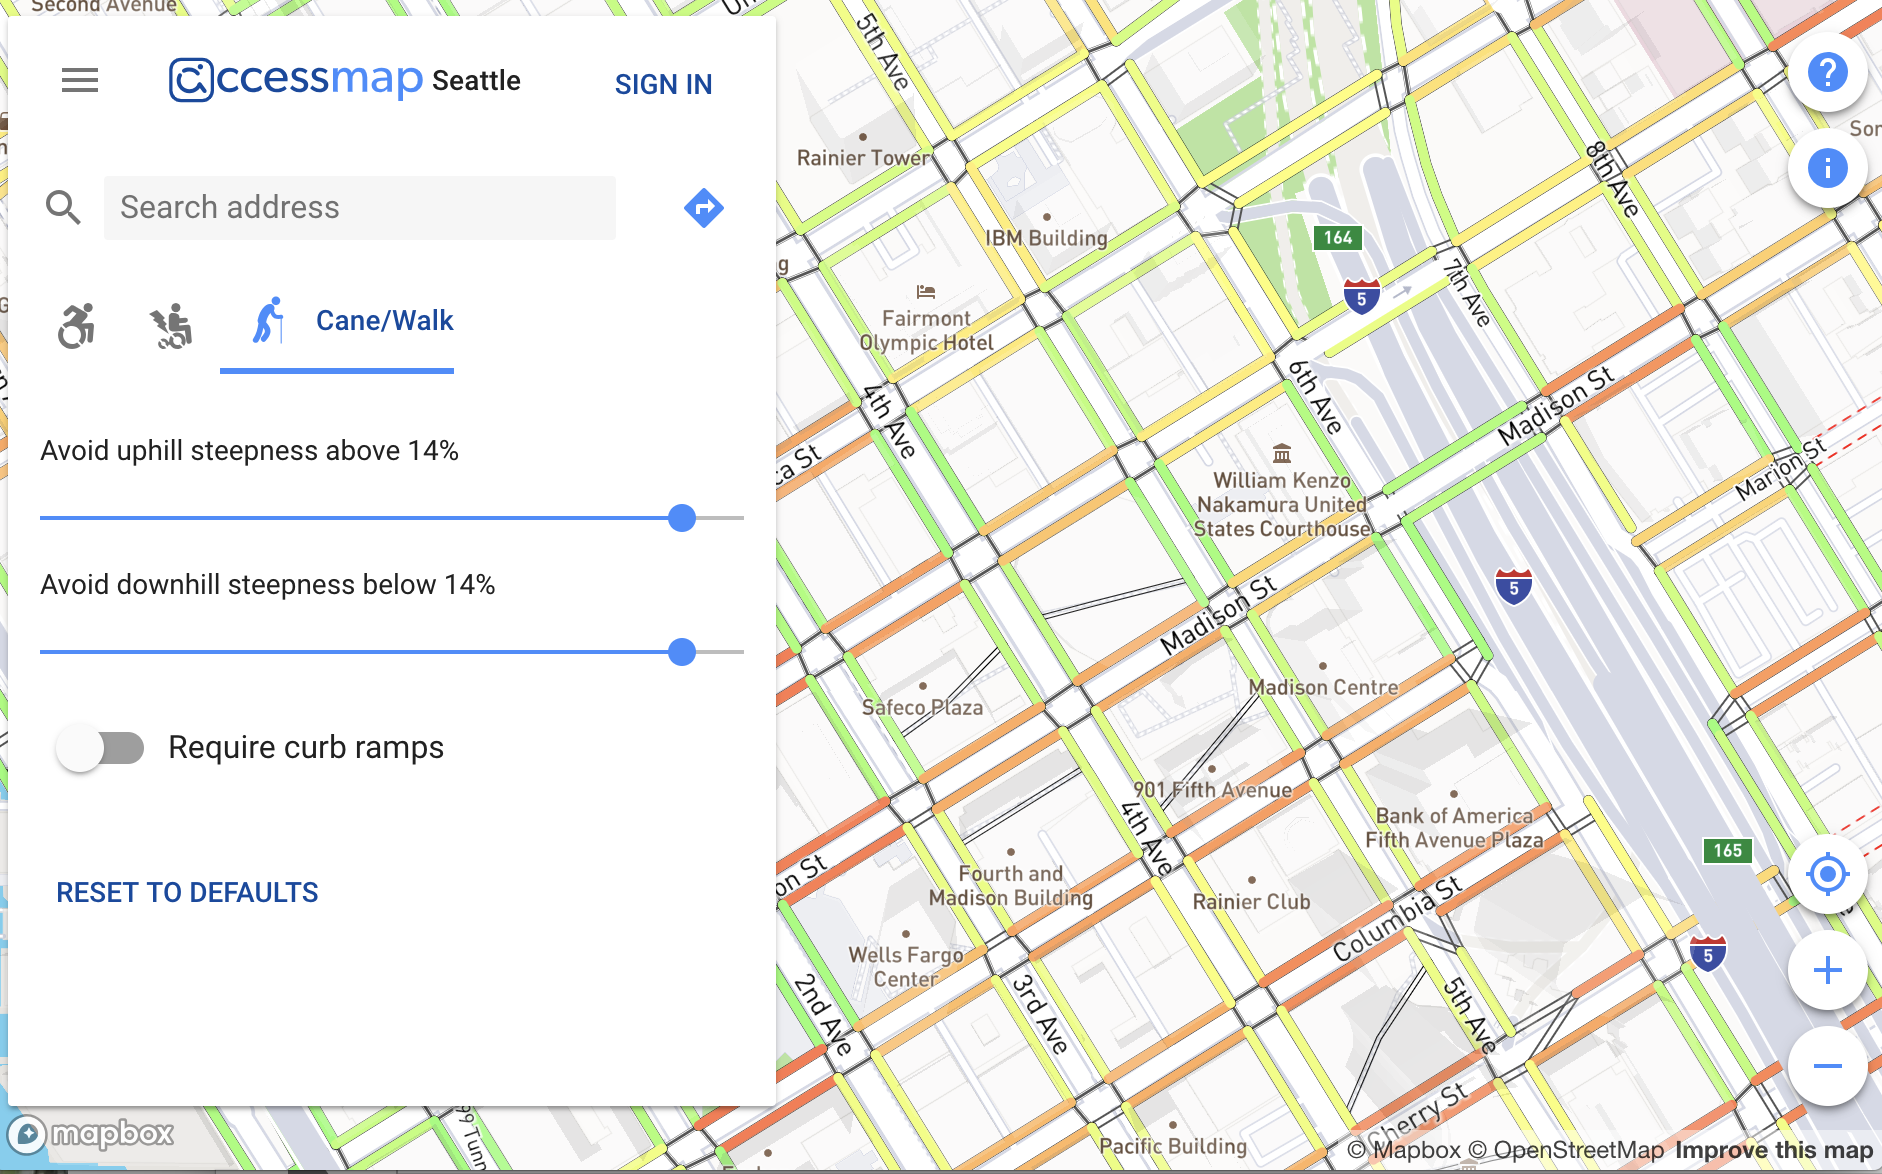
\includegraphics[width=5in]{pics/accessmap.png}
    \caption{AccessMap Screen Shot}
    \label{fig:accessmap}
\end{figure}

AccessMap currently can produce parametrically designed maps that always show the most up to data open data (derived from OpenSidewalks) about a region. 

\subsubsection{Proposed Development}

Operating hand-in-hand with AccessMap and OpenSidewalks (two projects discussed below), the goal of our work is to extend AccessMap to support users to automatically generate a custom 3D map model of any given area.  That model could then be printed at home, brought to a local library, or sent to a 3D printing service for relatively quick and inexpensive map production.  Beyond customizable map locations, ultimately the application would allow users to specify different scales and map features that are important to them.  

We will base our tactile design features on the comprehensive set of tactile map graphic symbols adopted by Braille Authority of North America (BANA) as created by (\cite{lobben2012tactile}, p. 107).% integrated into data driven design development tools and made available and consumable to landscape architects

%Anat: I commented this text out because I don't think it is product focused enough for NIDILLR's FIP in development. 
%The Tactile Maptile project designed the set of associated atomic symbols for that critical information.  Not only does this have implications for the map tiles specific to this project, but also more broadly works towards elevating pedestrian infrastructures in the context of our digital landscape.  This is important from a navigational perspective, but is also a reflection of the information designers, planners, and policy makers depend on to make significant decisions that affect our urban fabric.  Informed decisions based on incomplete data are not only difficult but also more prone to error and bias.  As we move rapidly towards sensor laced smart cities, it is critical these gaps be identified and understood in order to account for this influence on design and decision-making.  As such, this work is meant to take an accessible approach to data as it relates to pedestrian design and experience.

%Illustrative documentation of both the process and analysis that went into making these maps is directed more squarely at the design community. This project re-examines the pedestrian environment, with a focus on the specific needs of the low vision and blind communities. The goal of this work is to persuade designers to consider a broader spectrum of experience, and engage more critically in what it means to be designing inclusive cities.  

%This project is meant to bring attention to the deficiencies of the system currently place, in which accessibility checklists too often are accepted in lieu of truly inclusive design.  The straightforward approach is intended to remind designers that accessible design is good design, and if we want to build more equitable cities that means there is a huge spectrum of experiences we must first understand. 

\subsubsection{Validation}

\jm{ All studies need the following subsections to conform to the RFP:
\paragraph{Sample}
\paragraph{Environment}
\paragraph{Test Trials}
}

\ac{ needs writing


Our solution combines simple accessible interfaces with complex data integration and smart routing. To our users, the entire solution will be seamlessly presented in a workflow through which the travelers access a website, select the area of travel, the type of travel they wish to undertake in the area and travel preferences. The travelers are given the opportunity to verify the map location and features \textit{via} non-visual text-based exchange before printing the map.
% means what? A: means that in our UI pilot we found one of hardest things with building this UX/UI is ensuring that the tactile map model they got isn't of [Paris, Texas] when they actually meant [Paris, France]

The entire exchange is enabled and specifically designed for a portable 14-cell Braille-display. At the end, the traveler receives access to a downloadable 3D model file, access to an online URL where the model can be accessed for a specified duration, the option to have the model printed and sent to the user for a fee, and the option to subscribe to email alerts regarding any changes to the mapped region in the digital map repositories. 

}



\subsubsection{Product 2: AccessMap Interface Validation: Iterative Design of Mapping Interface}
\label{sec:accessmap-studies}
Our product will enable Deaf-blind individuals and those who support them  to independently create custom maps. Our studies will help support iterative design as we  refine and improve this product over the course of the proposal.

\subsubsection{Study 1: Usability of Interface Extensions}
Our first study will demonstrate the basic usability and accessibility of the updated AccessMap Interface. Specifically, we will test four specific tasks: Creating an account; Searching for an address; Setting Personalization Parameters, and Generating a map; Generating a map of choice.

\paragraph{Sample} For this sample, we will recruit Deaf-blind individuals, since the accessibility of the system to that specific population is a necessary precondition for the impact of our product. 

\paragraph{Environment} This study will take place in a lab environment, since our focus is on ensuring basic usability.

\paragraph{Test Trials}
After being introduced to the study, participants will be asked to use a modified think-aloud protocol while using AccessMap to accomplish each of the tasks. Because the study will involve Deaf-blind participants, participants will be instructed to complete each task, pausing to communicate with us if they have questions or comments about the interface. The entire session will be video-recorded, and an interpreter will be present to support communication between participants and the experimenters. At the end of the study, participants will be given a brief survey to fill out where they can add further comments about their experience. 

The final task, Generating a map of choice, will be participants' opportunity to generate a map for a location of their choice that they would like to use. This map will be printed and mailed to participants for the final study, end-to-end system use, described below. 

\subsubsection{Study 2: End-to-end system use}
\label{sec:field-web}
\jm{test that they can produce a map on their own when they want and use it}
The goal of the final study is to see how participants use the system to independently generate and use maps. 

\paragraph{Sample}
This study will involve the same sample as the previous study: Deaf-blind individuals local to our University. In addition, we will advertise the study in all cities where AccessMap data exists \jm{xx anat: list of cities}. This will help to expand our sample. 

\paragraph{Environment}
This study will take place online. Participants will be asked to fill out a survey the first and second time they use Accessmap. In addition, with their permission, we will log all interactions with the system.  Lastly, we will interview participants about their experience, and what happened when they received the physical map they requested (including how they used it and whether they used it). 

\subsubsection{Input from Stakeholders}
\label{sec:stakeholder-input}
\label{sec:stakeholder-input}
In this section we describe the activities of our Community of Practice, our ongoing participatory design stakeholder group. We describe how input will be collected from key stakeholders (including people with disabilities) to guide development activities.

While input from several expert users was incorporated throughout the design process of both the maps and the web application, a formal review of the maps produced thus far has not been conducted. 


The Community of Practice Activities will result in data collection of performance metrics that will allow us to validate the specific development goals as well as perform the overall project evaluation.

The following Community of Practice activities will be pursued within the development period:

\subsubsection{Early Development Baseline Survey}
\label{test:baseline}
Many of the individuals who are Deaf-blind and registered with the Deaf-Blind Service Center in Seattle are already familiar with our tactile map project. To assess our project impact beyond the local region, we will send out a survey to as many individuals as we can reach with the goal of understanding the current reach, cost, accessibility, reproducibility and information content in the tactile maps currently available to Deaf-blind travelers. We will also survey participants about other ways they access geographical, landscape and transit information. 

In this survey instrument, participants will be asked for their:  Age Bracket; HH Income Bracket; Disability Status; HH Size; Number of times tactile maps were used for trip planning in last month; Number of times tactile maps were used for trip planning ever; Cost of tactile maps; Time to creation of tactile maps (if they've had them created for them); Perceived cost of tactile maps; Perceived utility of tactile maps; Perceived eagerness to use tactile maps if they were accessible; Perceived need for improved navigational tools; Perceived need for improved connectivity; For the last 5 trips outside their home: Origin, Destination, Trip Purpose, Departure Time, Number of Modes Used, First-mile Mode, Last-mile Mode;

\subsubsection{Surveys of user groups: alpha and beta population}
\label{test:usersurvey}

These surveys will be implemented twice through the development period, with an alpha populations of 10 users and a beta population of at least 20 users.  
The content of the survey will generally be the same both times. The material covered by the survey is indicated below:
Individual travel patterns
 Age Bracket; HH Income Bracket; Disability Status; HH Size; Number of times tactile maps were used for trip planning in last month; Number of times tactile maps were used for trip planning ever; 
 Basic travel needs including:
Home Location
Up to three common destinations
Response to the user interaction
Response to accessibility, reliability and cost 
Solicited input on how outputs could be improved
Solicited input on how interaction could be improved
Response to the presence of customization options in the Tactile Map Tile planner
Perception of utility of real-time information presented by the update alerts
Perception of utility of information to overcome transportation and pedestrian challenges
Perception of accessibility of information 

Data Collection Period:
The Alpha User Group will be surveyed once the optimization algorithm development is completed and users can produce different maps for exploration only.
The Beta User Group will be surveyed once the production development of the pipeline is completed and the primary development of the optimization is completed for all trip types.

\ac{

In-person interviews
Understanding of information content in the maps
improvements in understanding, mental model of the terrain, satisfaction and feedback. Also used as metrics would be survey questions designed to assess the perception of accessibility and reproducibility
}

\subsubsection{Observational Field Studies: Alpha and Beta populations} 
\ref{test:fieldtest}
These observational field studies will be implemented twice through the development period, with an alpha populations of 10 users and a beta population of at least 20 users. These will be the same populations surveyed by the survey tool in Section \ref{test:usersurvey} so we can match their experience with their qualitative opinion of their experience.

We will invite members of Seattle’s Deaf-blind community to sessions at locations they frequent in the pilot areas. 
Participants will be asked to use the interface to make 4 different maps with different parameters and type of travel designation for each of those maps. 


Participants will then be asked for feedback on several map styles, and will also be surveyed on their informational needs and preferences.  


our proposed work includes recruiting and testing with Deaf-blind individuals \ref{sec:lab-tests}, and resolving remaining challenges in optimization \ref{sec:optimization}.
\item[Testing in Natural Contexts (Proof of product)] Our proposed work also includes field studies. We will be testing the map in use in field settings \ref{sec:field-map}, and testing the entire system (including web-based map creation) in the field \ref{sec:field-web}. 


\subsubsection{Midway Input: Presentation of Working System}

\jm{xx describe some sort of midway input opportunity} 

\subsubsection{Summative Input: Presentation of Final System}

\jm{explain how our final report will include some sort of focus group at the end with reactions to what we've done?}

\subsubsection{Stage of Development and Specific Plan}
\label{sec:stage}


    


%\subsection{Enabling User to Produce Maps Themselves (Mankoff)}

\subsection{Conclusion}
% needed?
% LocalWords:  customizability

Mobility and orientation are among the biggest challenges for visually impaired people.
This project addresses a critical need of making available information about mobility and transportation to a cohort that has been excluded from a growing body of timely knowledge on which the majority of citizenry rely to access mobility.
This project presents an alternative approach to understanding the pedestrian experience of individuals who have both vision limitations and impacted hearing, a growing subpopulation among the aging population. 
We have learned from our prior work that it is important to identify scalable ways in which pedestrian environments and transit routes are encoded in tactile forms, and given the specific constraints of the population, it is important to provide a simple, cost-effective way to accessing this information.
Through optimizing the tactile readability of the maps, we can help change the pedestrian navigation experience and assist in planning for The Complete Trip. Our system is a tool that will enable users to create their own maps independently, and to navigate independently. This in turn will maximize their independence and improve their inclusion into society, access to employment, and ultimately their economic and social self-sufficiency. 

